


\chapter{Browse: Macaron}
\label{ch:macaron}

\begin{figure}[htbp]
\begin{center}
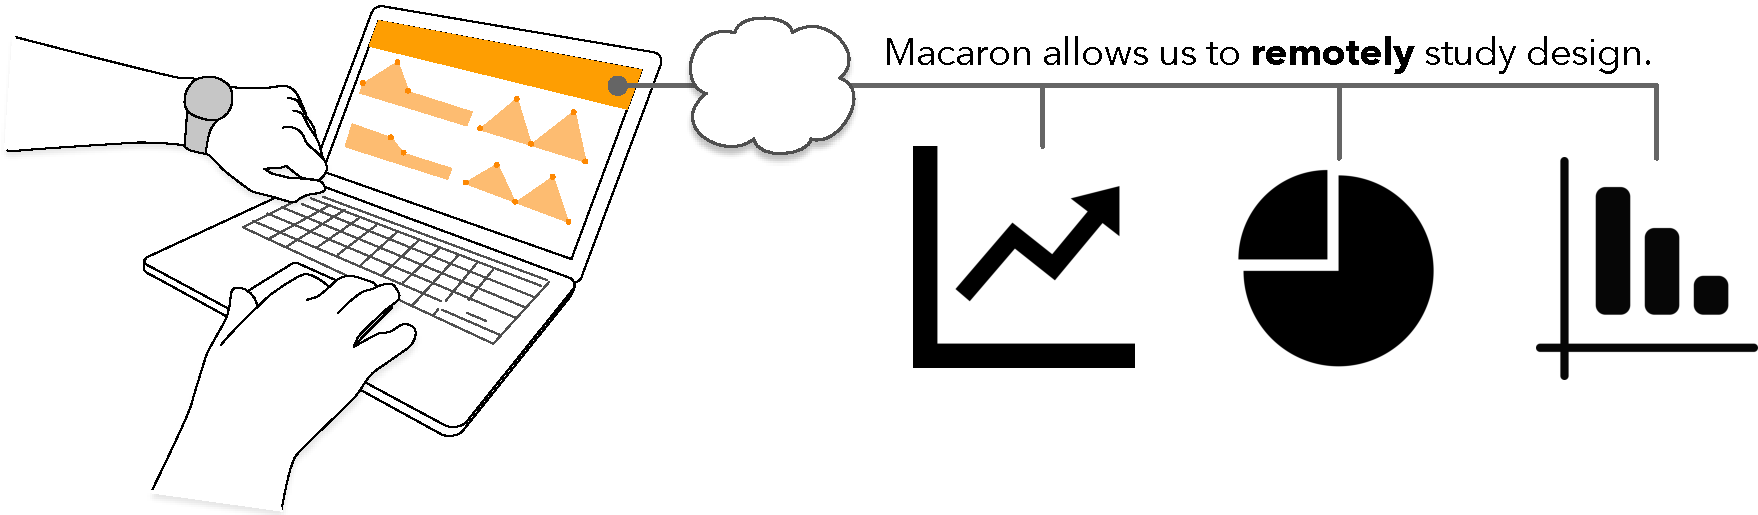
\includegraphics[width=0.9\textwidth]{poster/MacaronPoster-HS16-conceptsketch-words}
\caption{Concept sketch for a Macaron, an online, open-source VT editor features incorporable examples and remote analytics.}
\label{hapticexamples:designgallerysketch}
\end{center}
\end{figure}

\noindent
\inlineHeading{Preface} 
In our third vibrotactile design tool, Macaron\footnote{\fullCitation{Schneider2016macaron}}, we explored the design activity of \emph{browsing} external examples.
%In Chapters \ref{ch:hapticinstrument} and \ref{ch:tactileanimation}, our participants used personal experience and sought tools for reuse.
Because we explored \haxd tool implementation in-depth in \autoref{ch:tactileanimation}, we knew how to build Macaron; we thus focused on studying the design process\osE{. We} specifically \osE{investigated} how different ways of viewing or reproducing elements of a vibrotactile icon affects design.
We based this task on the effective sound-based task in \autoref{ch:tactileanimation}\osE{:} participants designed haptic tracks for visual animations.
\osE{To complement our previous studies,} participants were generally na\"ive to haptics and media design.
We used phenomenology and grounded theory methods augmented by logged user actions and visualized timelines to look at our participants' design process\osE{: we directly observed}
the different stages of design, including \emph{browsing}, \emph{sketching}, and iterative \emph{refinement}.


\section{Abstract}
Examples are a critical part of any design process,
but supporting their use for a haptic medium is nontrivial.
Current  libraries for vibrotactile (VT) effects provide neither insight into examples' construction nor  capability for 
deconstruction and re-composition.
To investigate the special requirements of example use for VT design, we studied designers as they used a web-based effect editor, \emph{Macaron}, which we created as both an evaluation platform and a practical tool. 
We qualitatively characterized participants' design processes and observed two basic example uses: as a starting point or template for a design task, and as a learning method.
We discuss how features supporting internal visibility and composition influenced these example uses, and articulate several implications for VT editing tools and libraries of VT examples.
We conclude with future work, including plans to deploy Macaron online to examine examples and other aspects of VT design \emph{in situ}.



\section{Introduction}

Creativity often sparks when an inventor, examining existing ideas, sees a way to combine them with a novel twist~\cite{Warr2005}.
% Creativity often sparks when the inventor sees a way to combine existing ideas with a novel twist~\cite{Warr2005}.
An environment rich with \emph{examples} is fuel for this fire. In industrial and graphic design \cite{Buxton2007,Herring2009} their use improves process and final results~\cite{Dow2011,Lee2010a}.

Several effect libraries are available to designers of vibrotactile (VT) sensations, e.g., for accessible wayfinding \cite{Zelek2003} or % rich 
media experiences \cite{SchneiderAsiaHaptics2014,Israr2014,ImmersionCorporation,Culbertson2014}. 
%\kmC{slc} % leave out Seifi2015? since it does not have all these limitations. use as positive example instead?
But despite the need for effect customizability~\cite{Seifi2014}, VT library elements are generally opaque in construction and immutable.
Recent advances include limited parameter adjustability~\cite{Israr2014,SchneiderAsiaHaptics2014} and faceted library search and browsing~\cite{Seifi2015}. 
Despite this, designers still must either choose a pre-existing sensation or build from scratch:
\textit{elements cannot be sampled, recombined, built upon or adapted}. %imitated with variations.
In contrast, web designers can access a page's source;
graphic and sound designers can sample and incorporate colours and sounds from other media.

%\begin{figure}
%        \centering
%        \includegraphics[width=0.5\textwidth]{MacaronScreenshotHi}
%        \caption{Macaron interface, ``\hi'' version featuring both composability (copy and paste), and visibility of underlying parameters. The user edits her sensation on the left, while examples are selected and shown on the right. One editor has focus at a time, shown by the red playhead. Examples are non-modifiable (keyframes cannot be inserted or moved).
%        Macaron is publicly available at \emph{{\tt hapticdesign.github.io/macaron}}.
%}
%        \label{fig:macaron:hi}
%\end{figure}


\begin{figure}
        \centering
%        \includegraphics[width=0.8\textwidth]{full/MacaronScreenshotHi}
        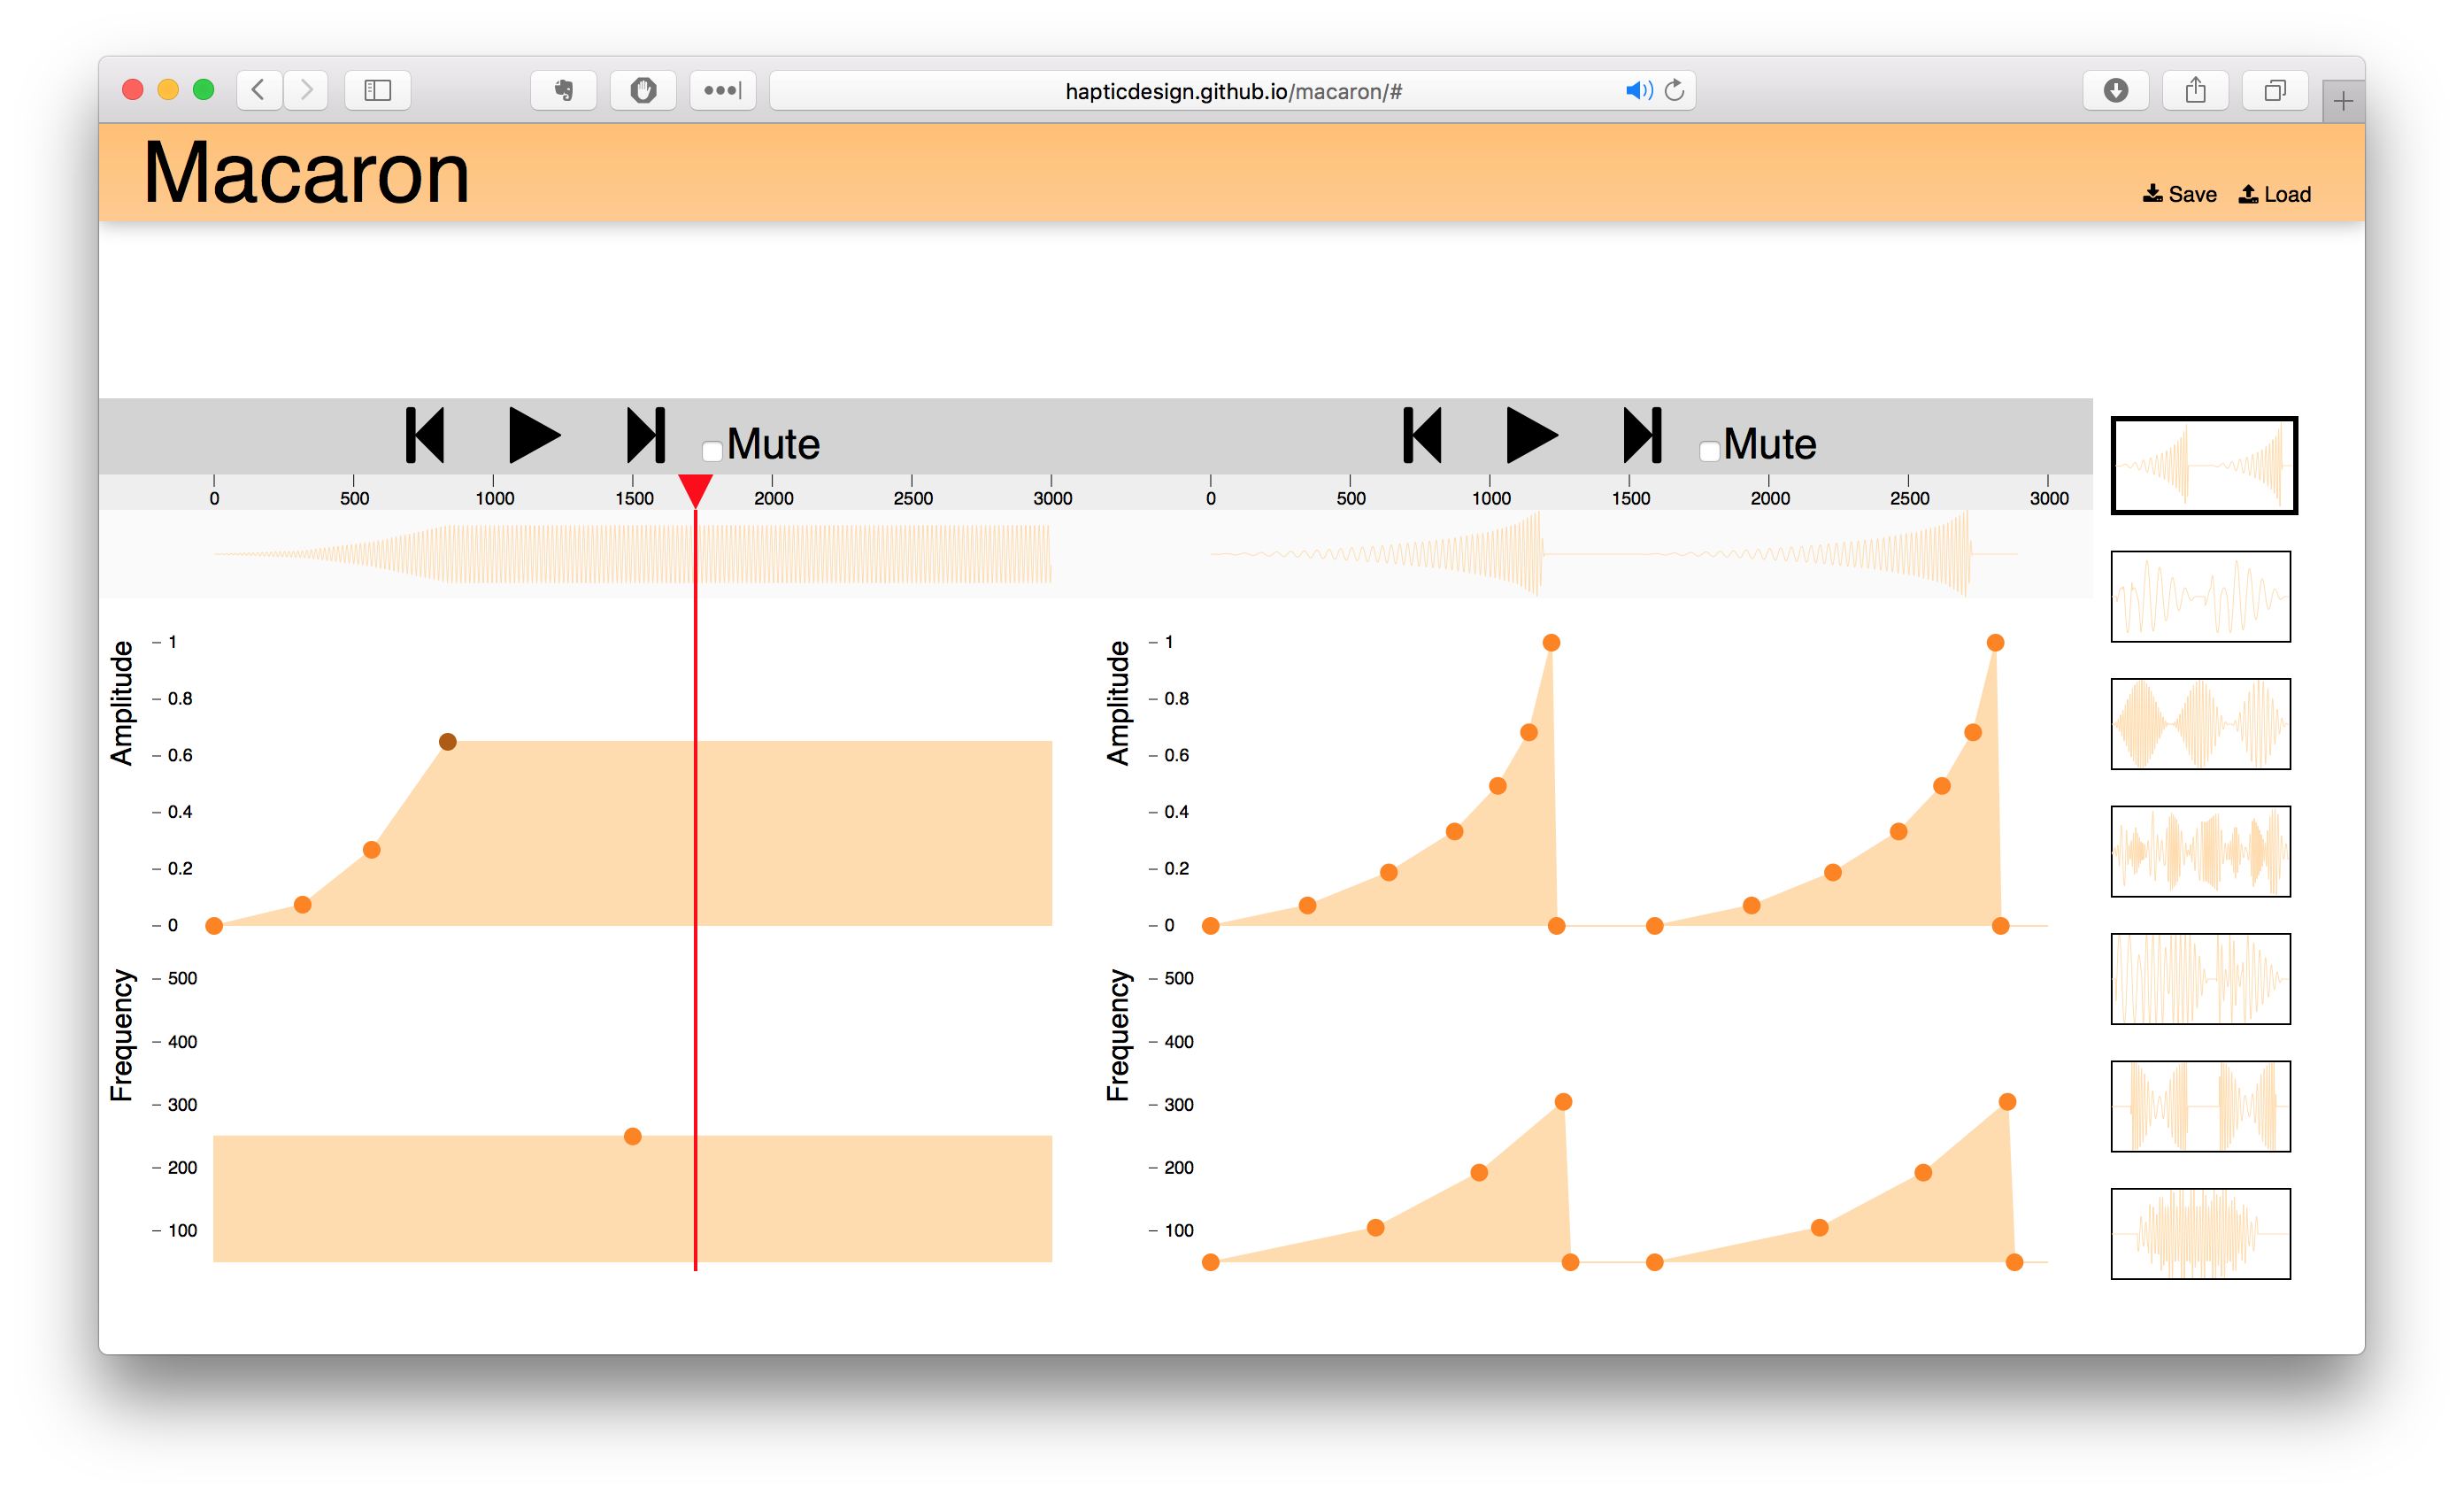
\includegraphics[width=0.9\textwidth]{poster/IMG-MacaronScreenshot-Poster}
        \caption{Macaron interface, ``\hi'' version featuring both composability (copy and paste), and visibility of underlying parameters. The user edits her sensation on the left, while examples are selected and shown on the right. 
%        One editor has focus at a time, shown by the red playhead. Examples are non-modifiable (keyframes cannot be inserted or moved).
        Macaron is publicly available at \emph{{\tt hapticdesign.github.io/macaron}}.
}
        \label{fig:macaron:hi}
\end{figure}




%\begin{figure}[tb]
%    \centering
%    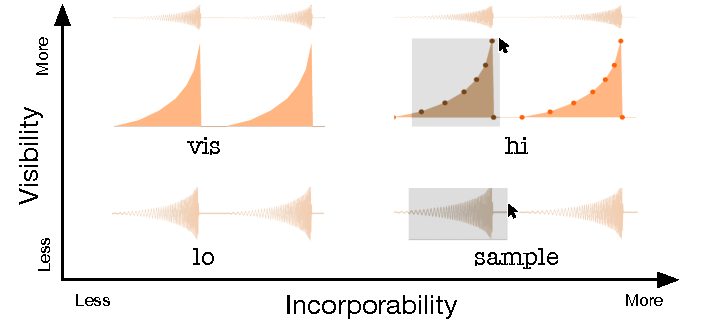
\includegraphics[width=0.8\textwidth]{VersionSpace-16-01-29}
%    \caption{Design space for Macaron versions. \hi and \select both allow for selection and copying of example keyframes. \vis and \hi both show the underlying profiles. \lo represents the current status quo; only a waveform is shown.
%    %\osC{slc}%"extraction/extractability"? ``sample-ability''?
%    %\kmC{slc} % 11.07 10:40 I'm getting weird shadowing in this one, pretty sure it's not right. If it is, I don't understand what I'm seeing. Also it's a big figure and may not be pulling its weight.
%    %OS: 02.01 I've adjusted contrast and shading issues. Does this look better?
%    }
%    \label{fig:versions}
%\end{figure}


Here, we \textit{examine the potential role of examples} in VT design, to establish how to best support their use.
% Here, we examine the role of examples in VT design.
We designed a web-based editor and interactive \emph{design gallery} \cite{Lee2010a,Marks1997} (\autoref{fig:macaron:hi}) for VT sensations,
then asked users to compare versions (\autoref{fig:versions}) that vary in example accessibility via \emph{visibility} and \emph{incorporability}, as they create VT effects for animations (\autoref{fig:animation}).
%\kmC{adequate grounding of this choice? slc} % KM 11.07 1227 as I come back later to these terms (in tool variant choice, then results) I realized there is not a lot of justification for choosing these dimensions. I think we had really good reasons for going this way, but it doesn't come across.

%We then compare versions of this tool which vary in power of examples use: the editor alone, relative to designer access to examples with low or high \emph{visibility} and low or high \emph{composability}.
Analysis of user action logs provide an objective picture of the VT design process. To validate the deployment of this methodology at scale, we also interpret and validate logs with direct observation and interviews.
Specifically, we:
\begin{itemize}
\item introduce \textit{Macaron}, a web-based VT effect editor through which examples can be used directly in designs,
\item find that \textit{visible, incorporable examples make design easier} by providing a starting point for design and scaffolding to learn how to work with VT parameters,
\item identify \textit{implications for future tools and libraries}, and
\item discuss the \textit{opportunities afforded by a web-based editor} as a practical tool and platform for studying other aspects of VT design at scale.
\end{itemize}











\newcommand{\macaronBigImageWidth}{0.55\textwidth}
\newcommand{\macaronSmallImageContainerWidth}{0.42\textwidth}
\newcommand{\macaronSmallImageWidth}{0.24\textwidth}


% \begin{figure*}[htb]
% % \centering
%     \centering
%         \begin{subfigure}{\macaronSmallImageWidth}
%             % \centering
%             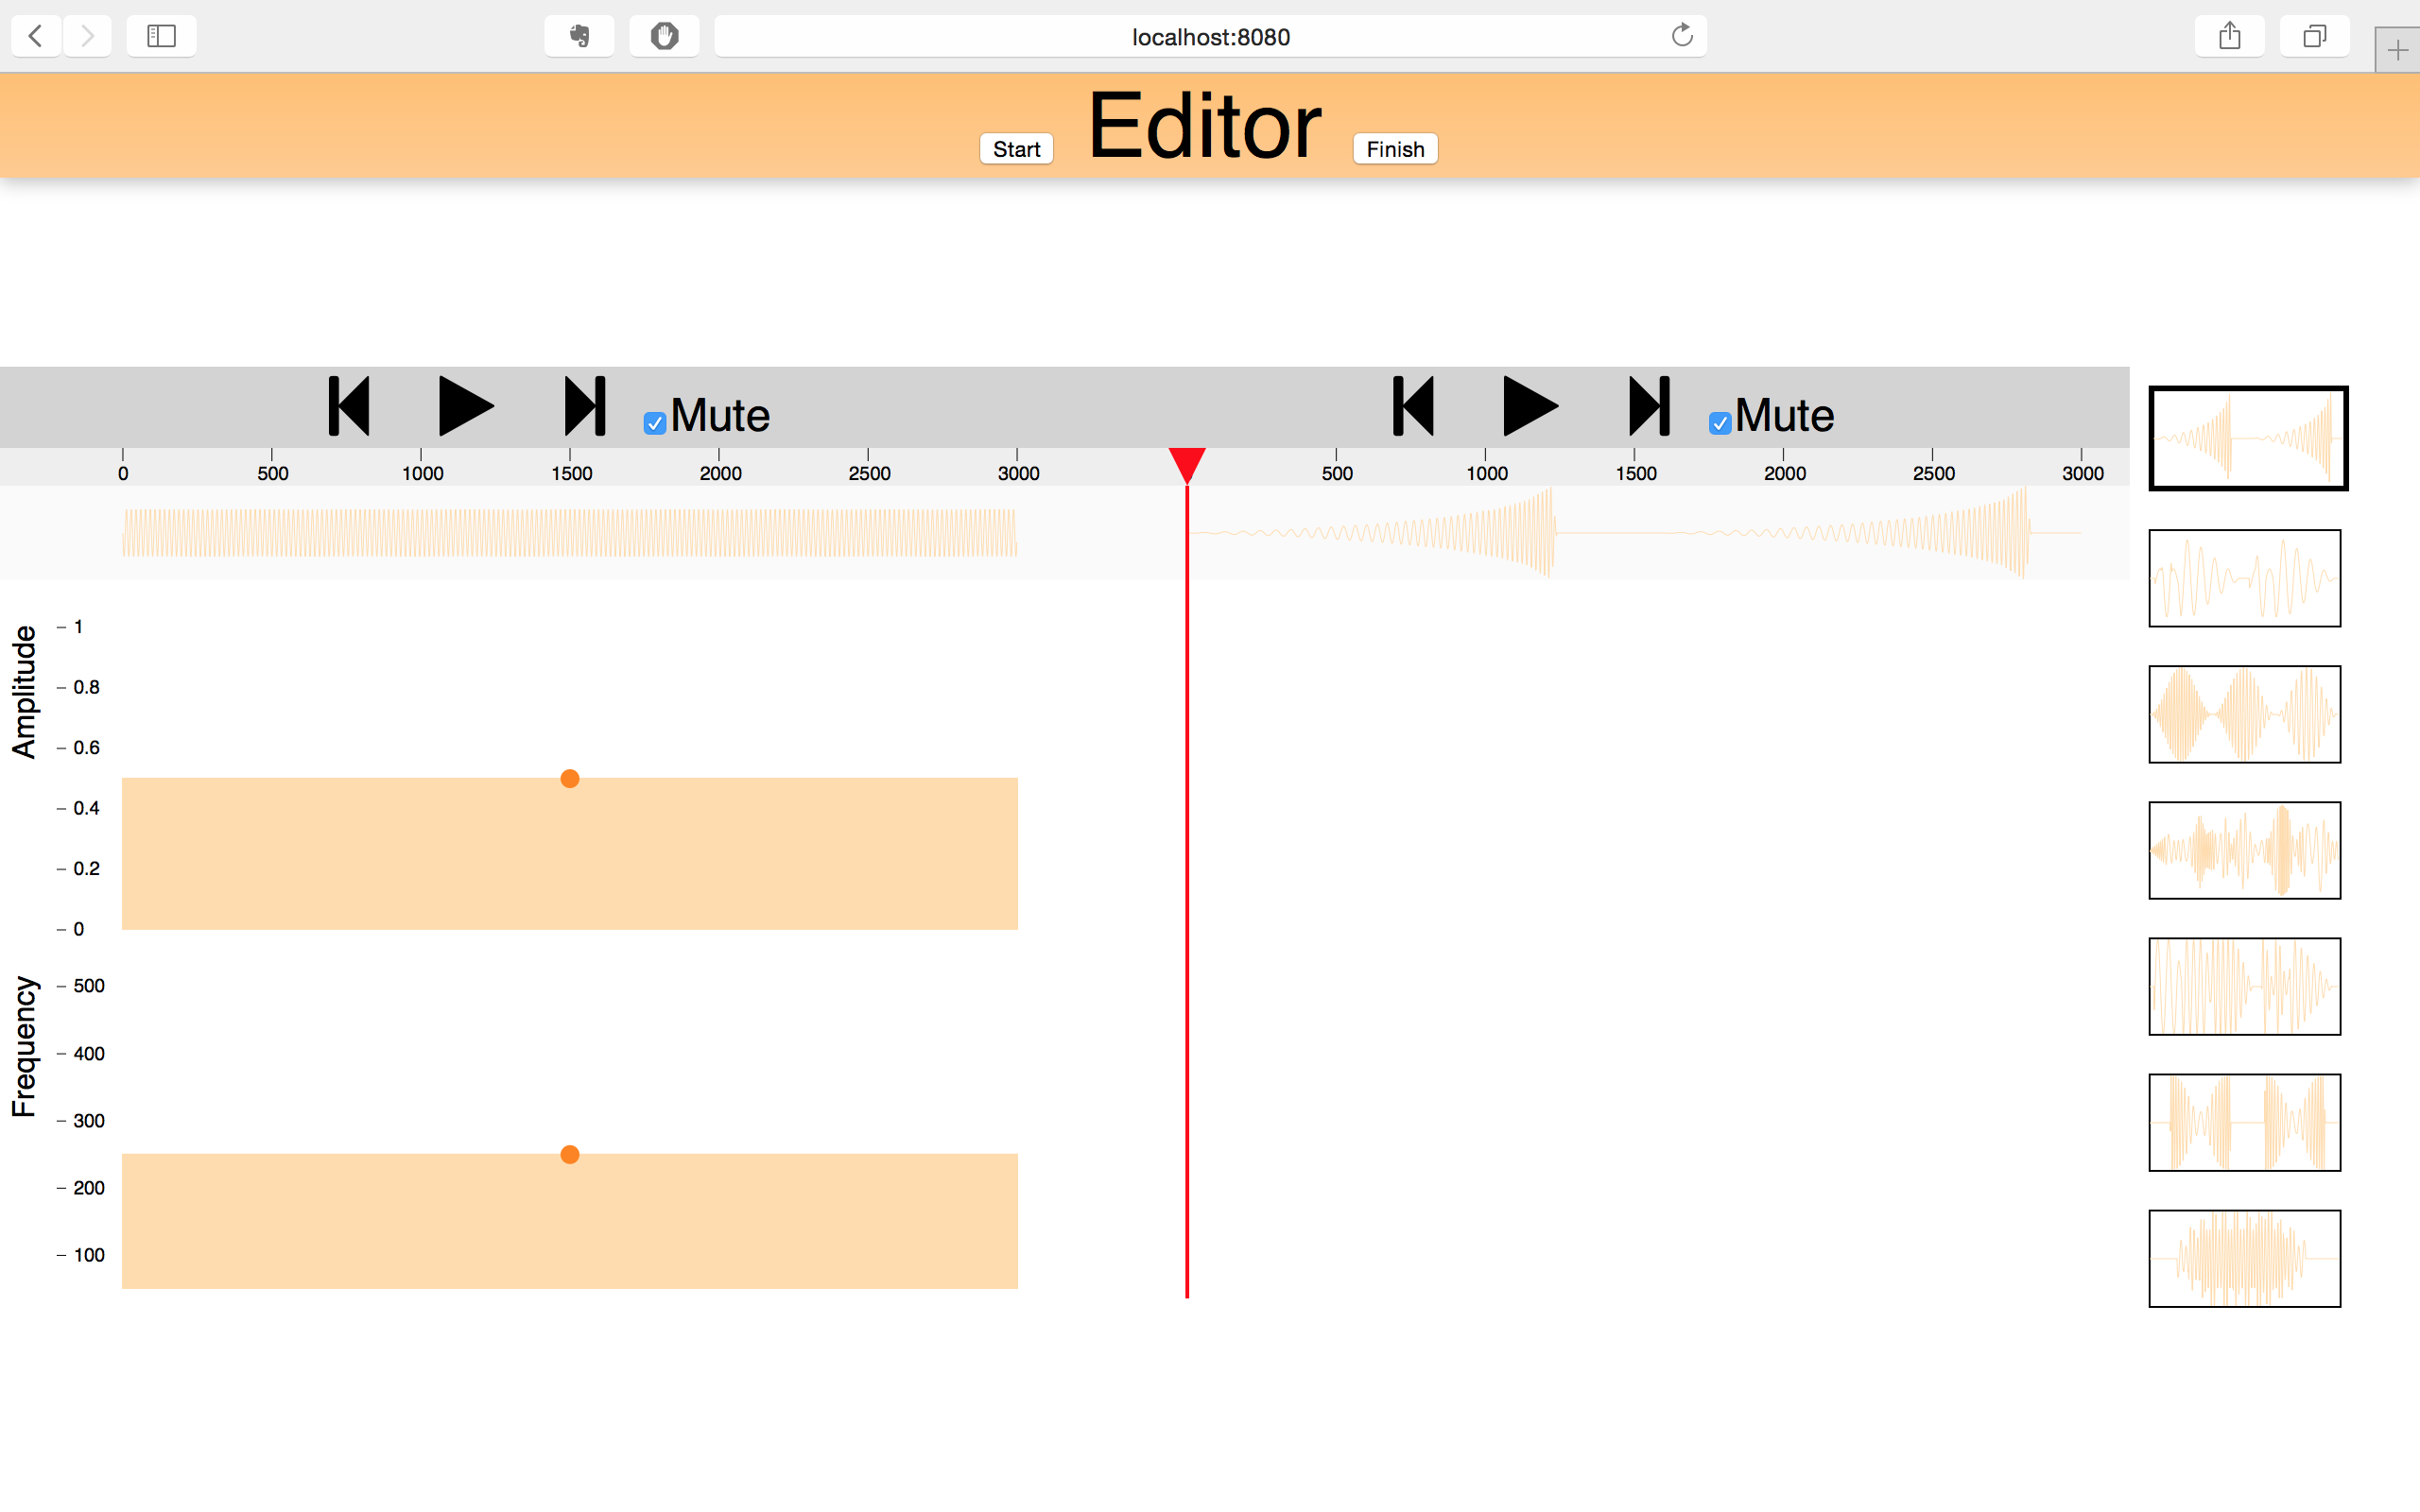
\includegraphics[width=\textwidth]{MacaronScreenshotLo}
%     	   \caption{\lo version.}
%     	   \label{fig:macaron:lo}
%         \end{subfigure}
%         \begin{subfigure}{\macaronSmallImageWidth}
%             % \centering
%             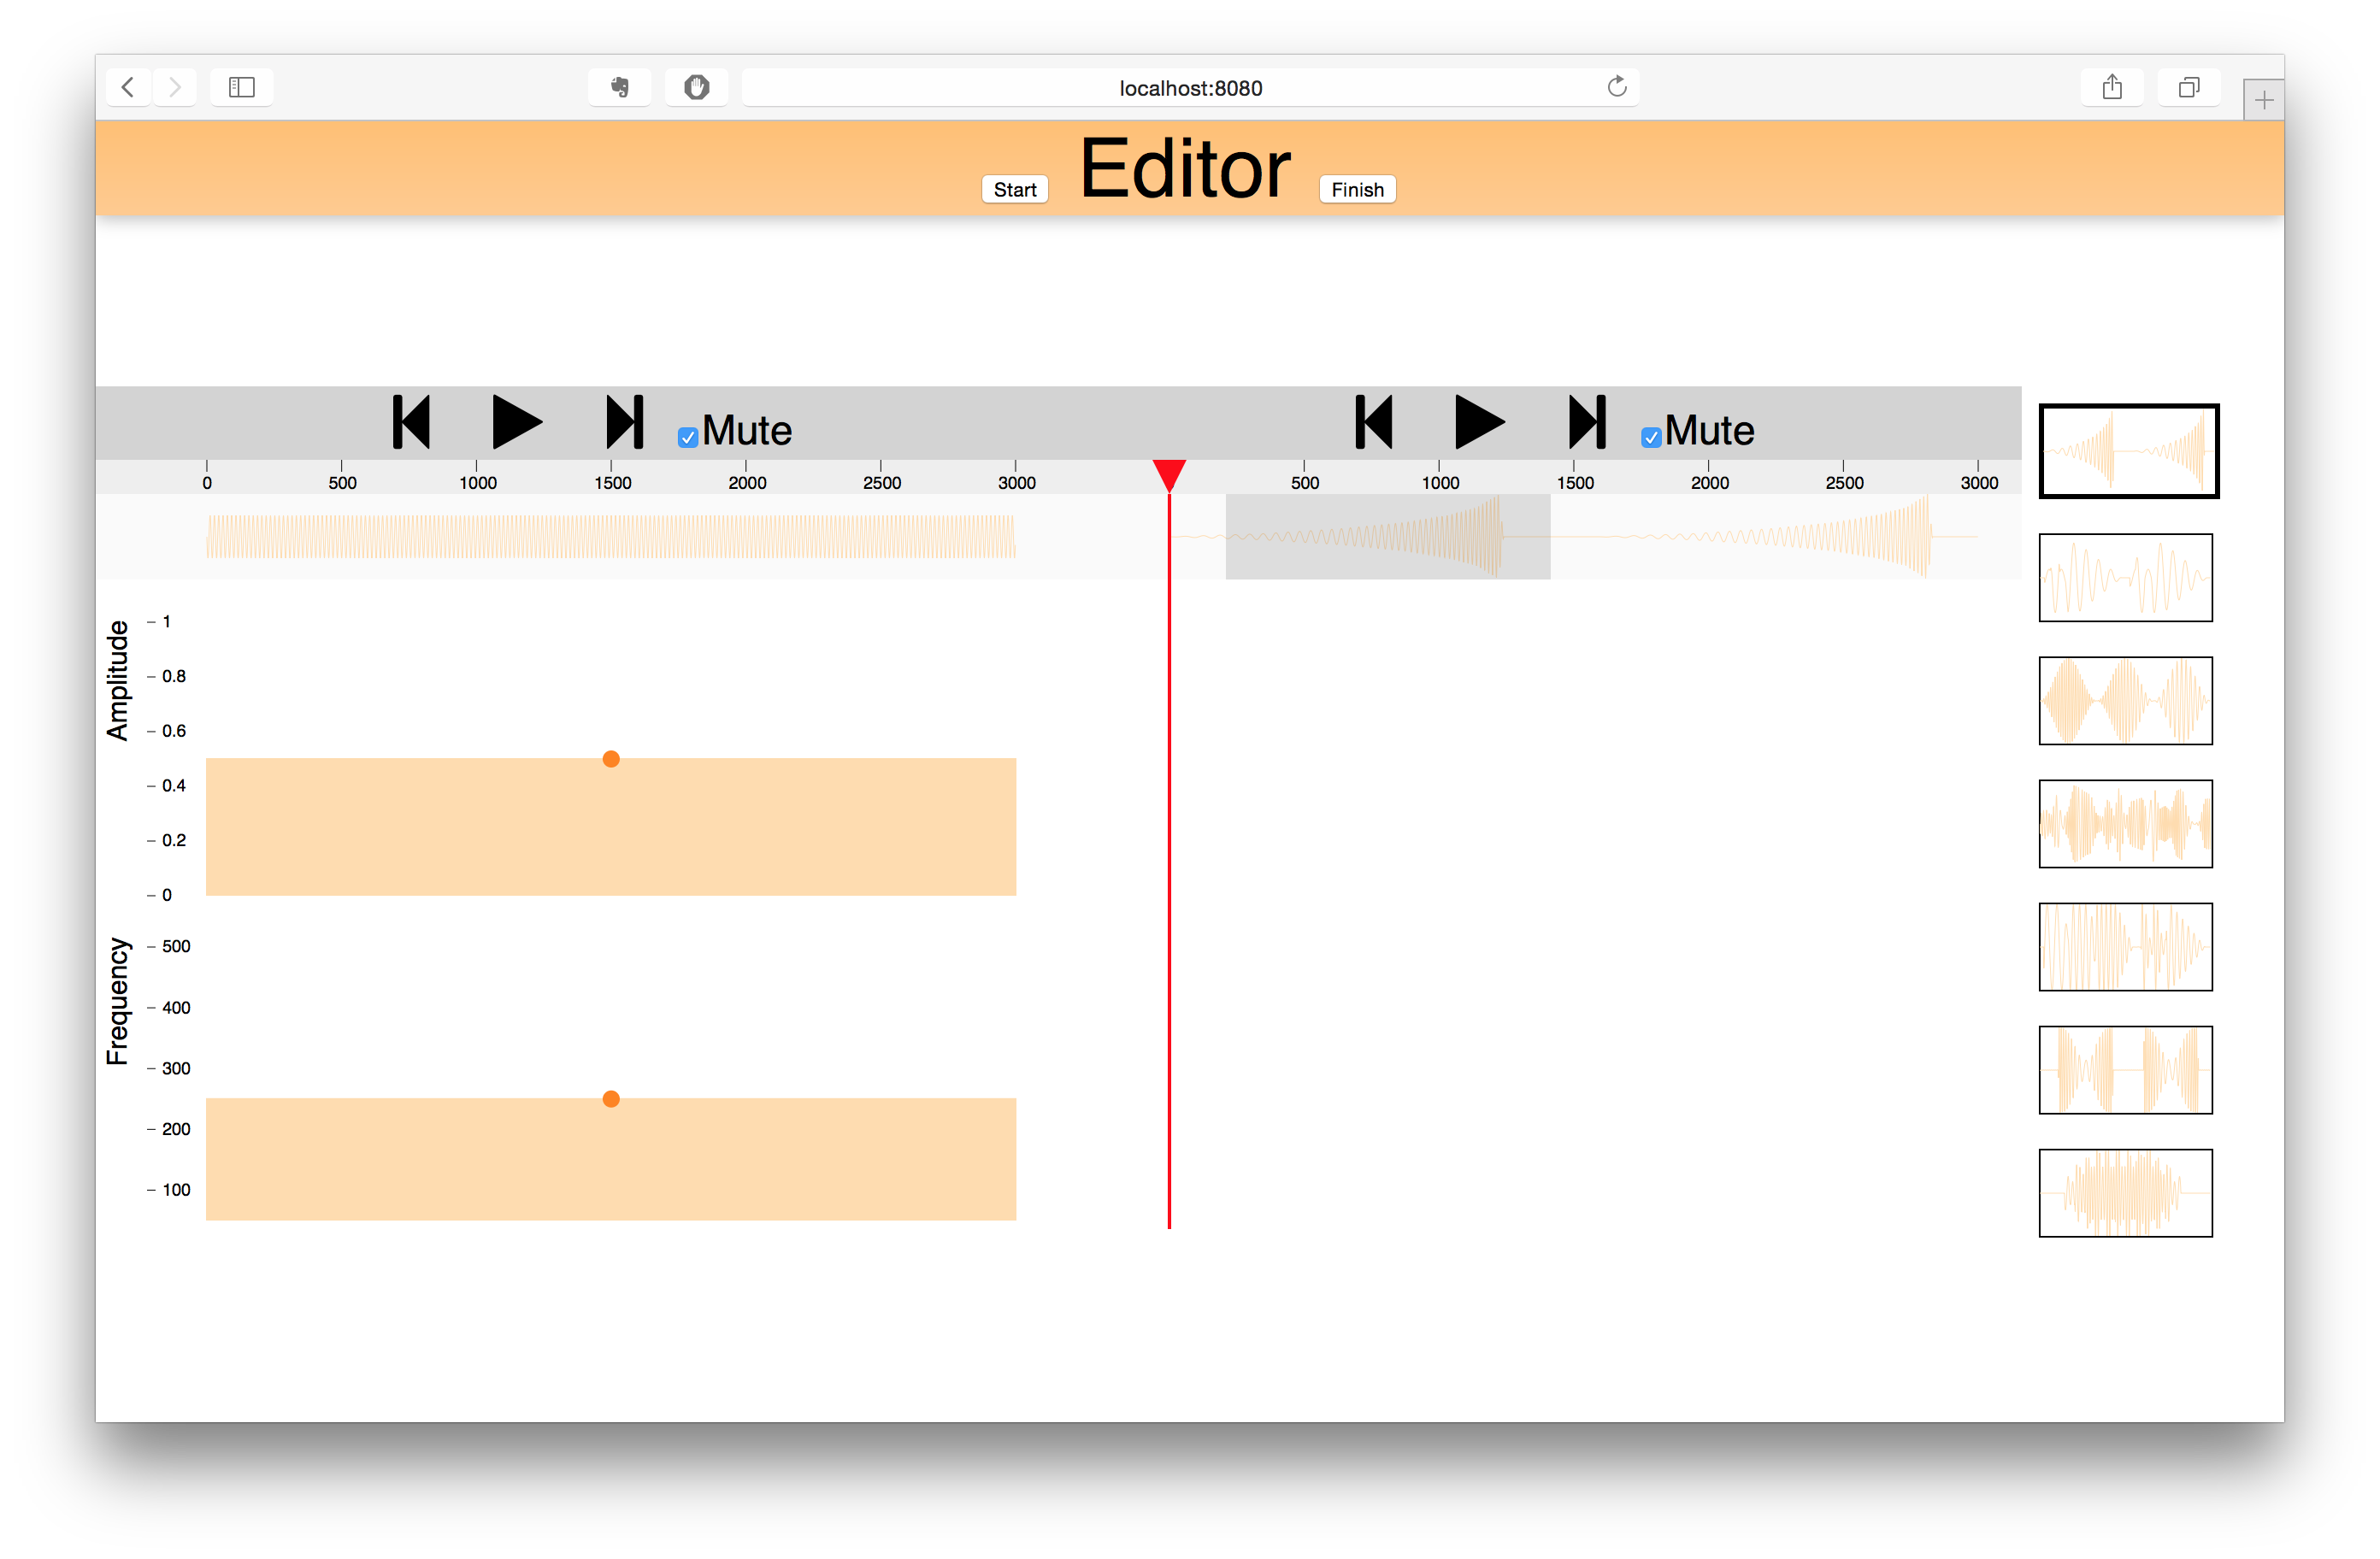
\includegraphics[width=\textwidth]{MacaronScreenshotSelect}
%     	   \caption{\select version.}
%     	   \label{fig:macaron:select}
%         \end{subfigure}
%         \begin{subfigure}{\macaronSmallImageWidth}
%             % \centering
%             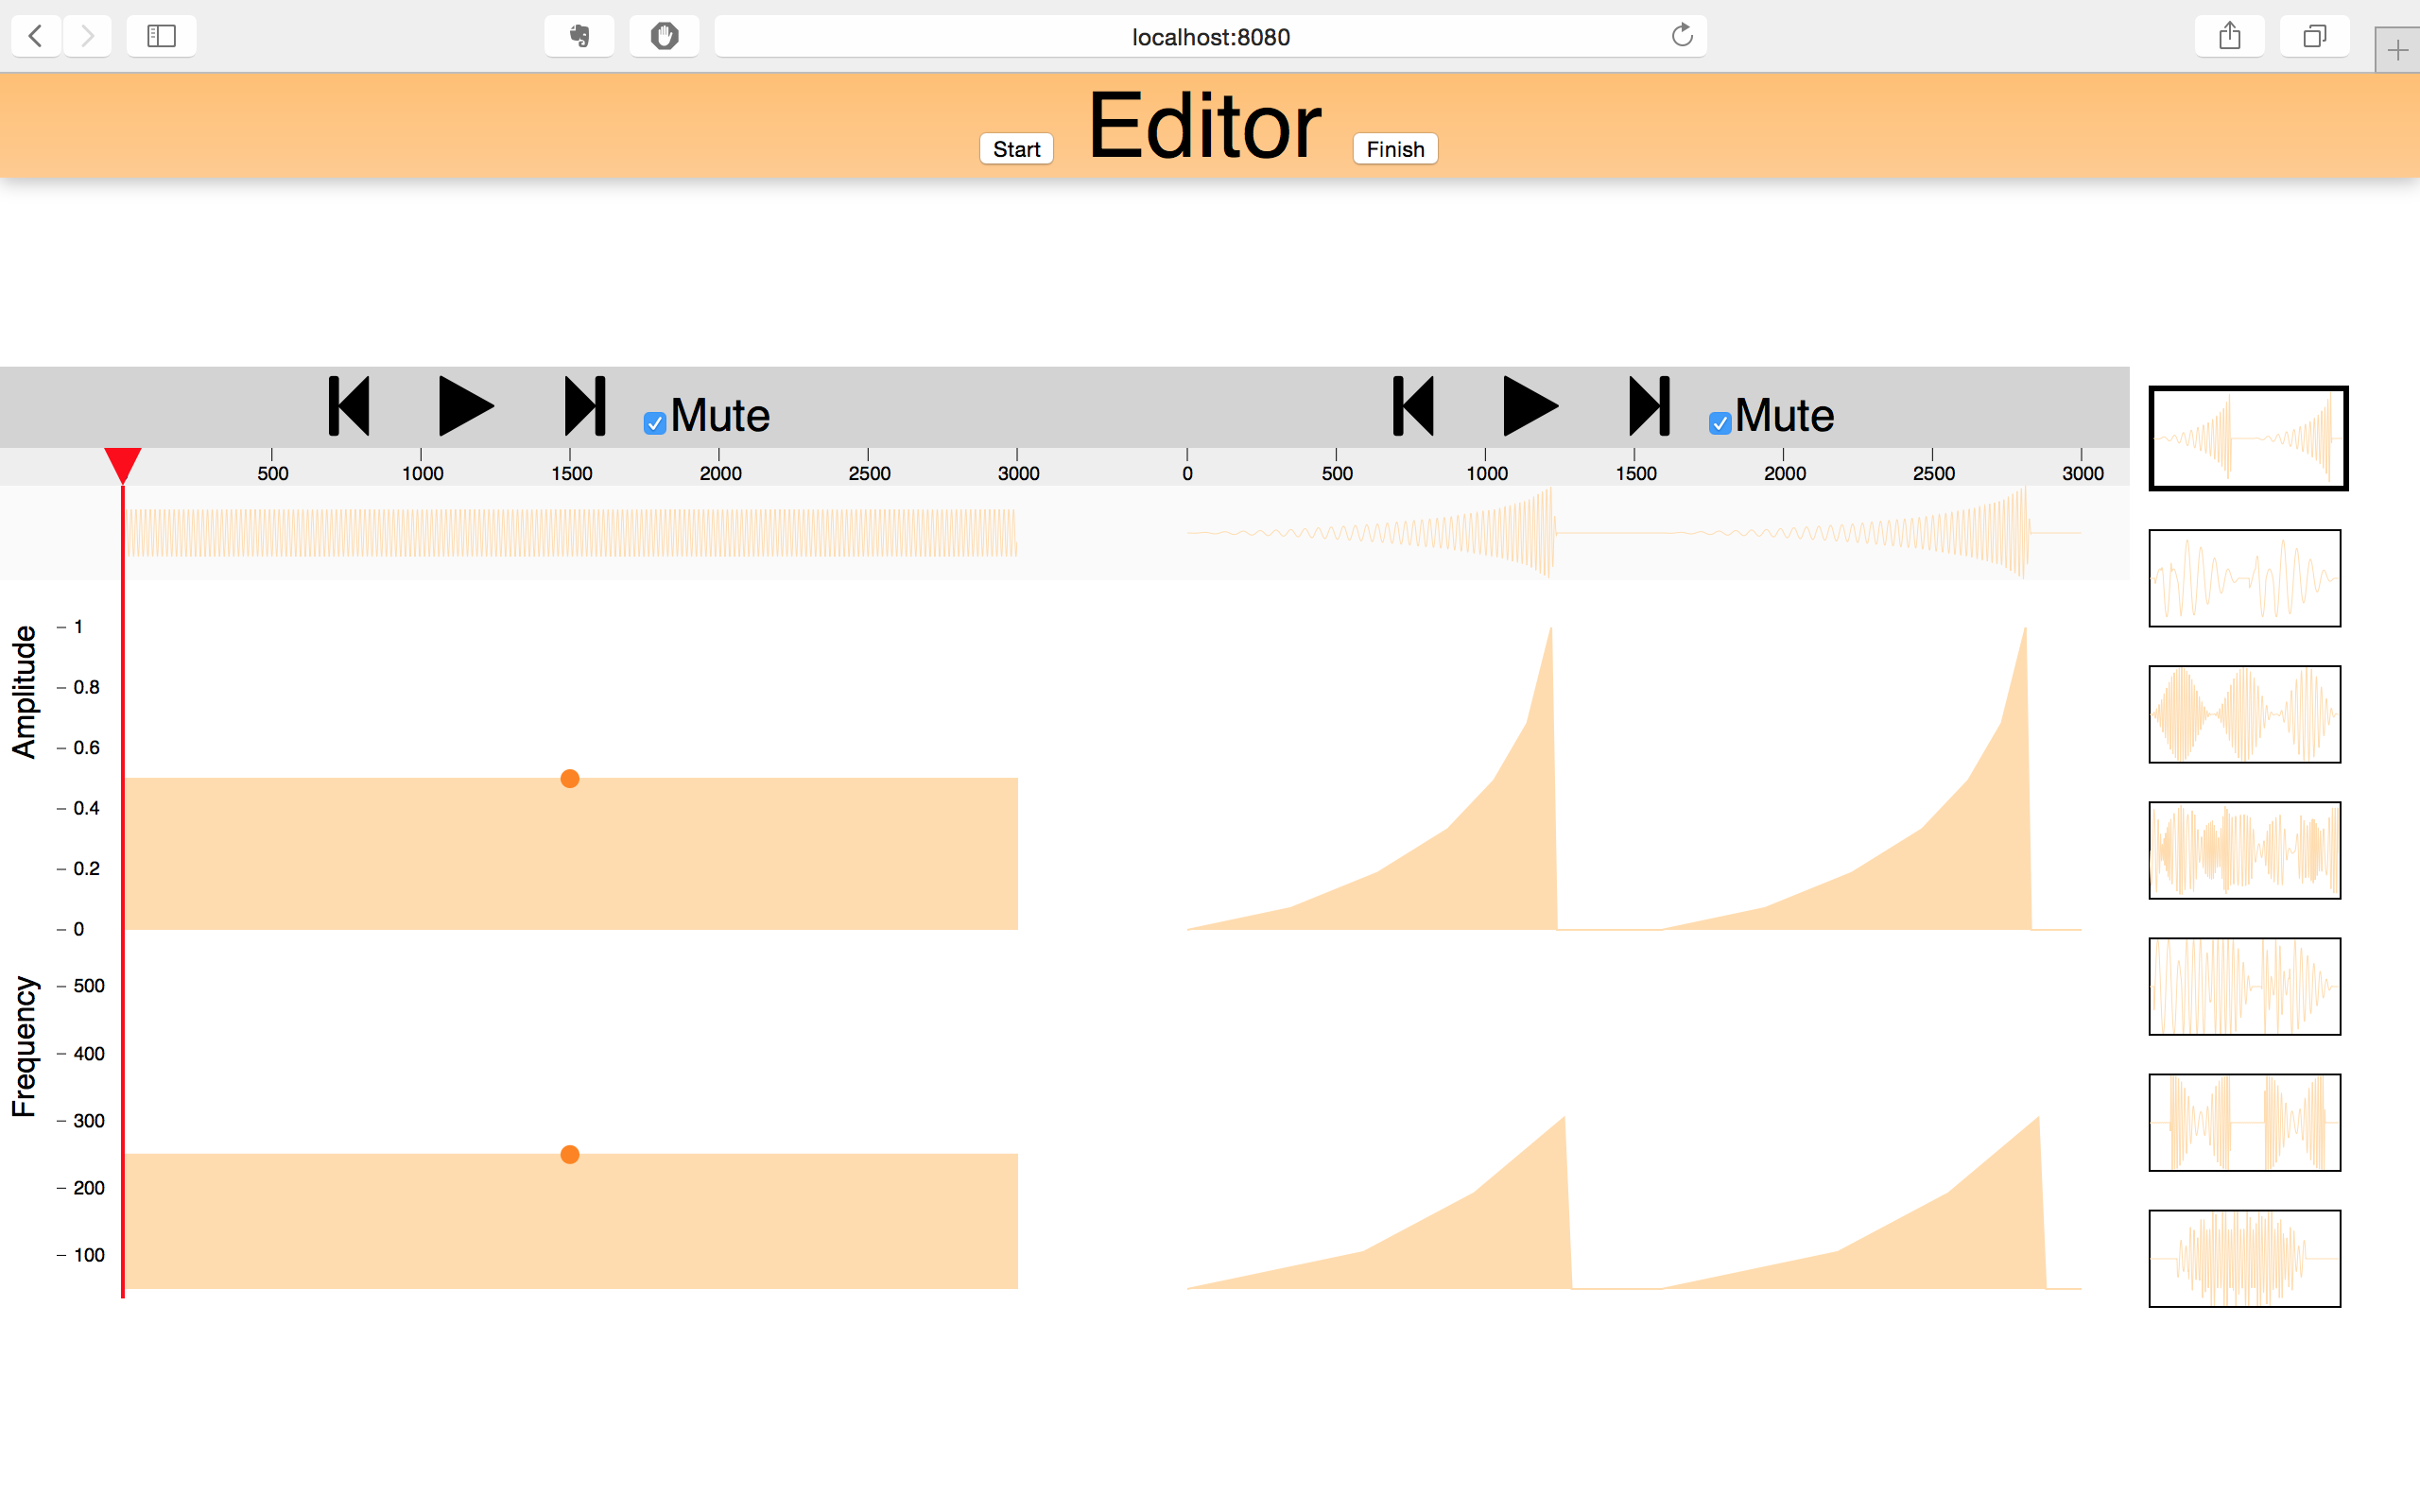
\includegraphics[width=\textwidth]{MacaronScreenshotVis}
%     	   \caption{\vis version.}
%     	   \label{fig:macaron:vis}
%         \end{subfigure}
%         \begin{subfigure}{\macaronSmallImageWidth}
%             % \centering
%             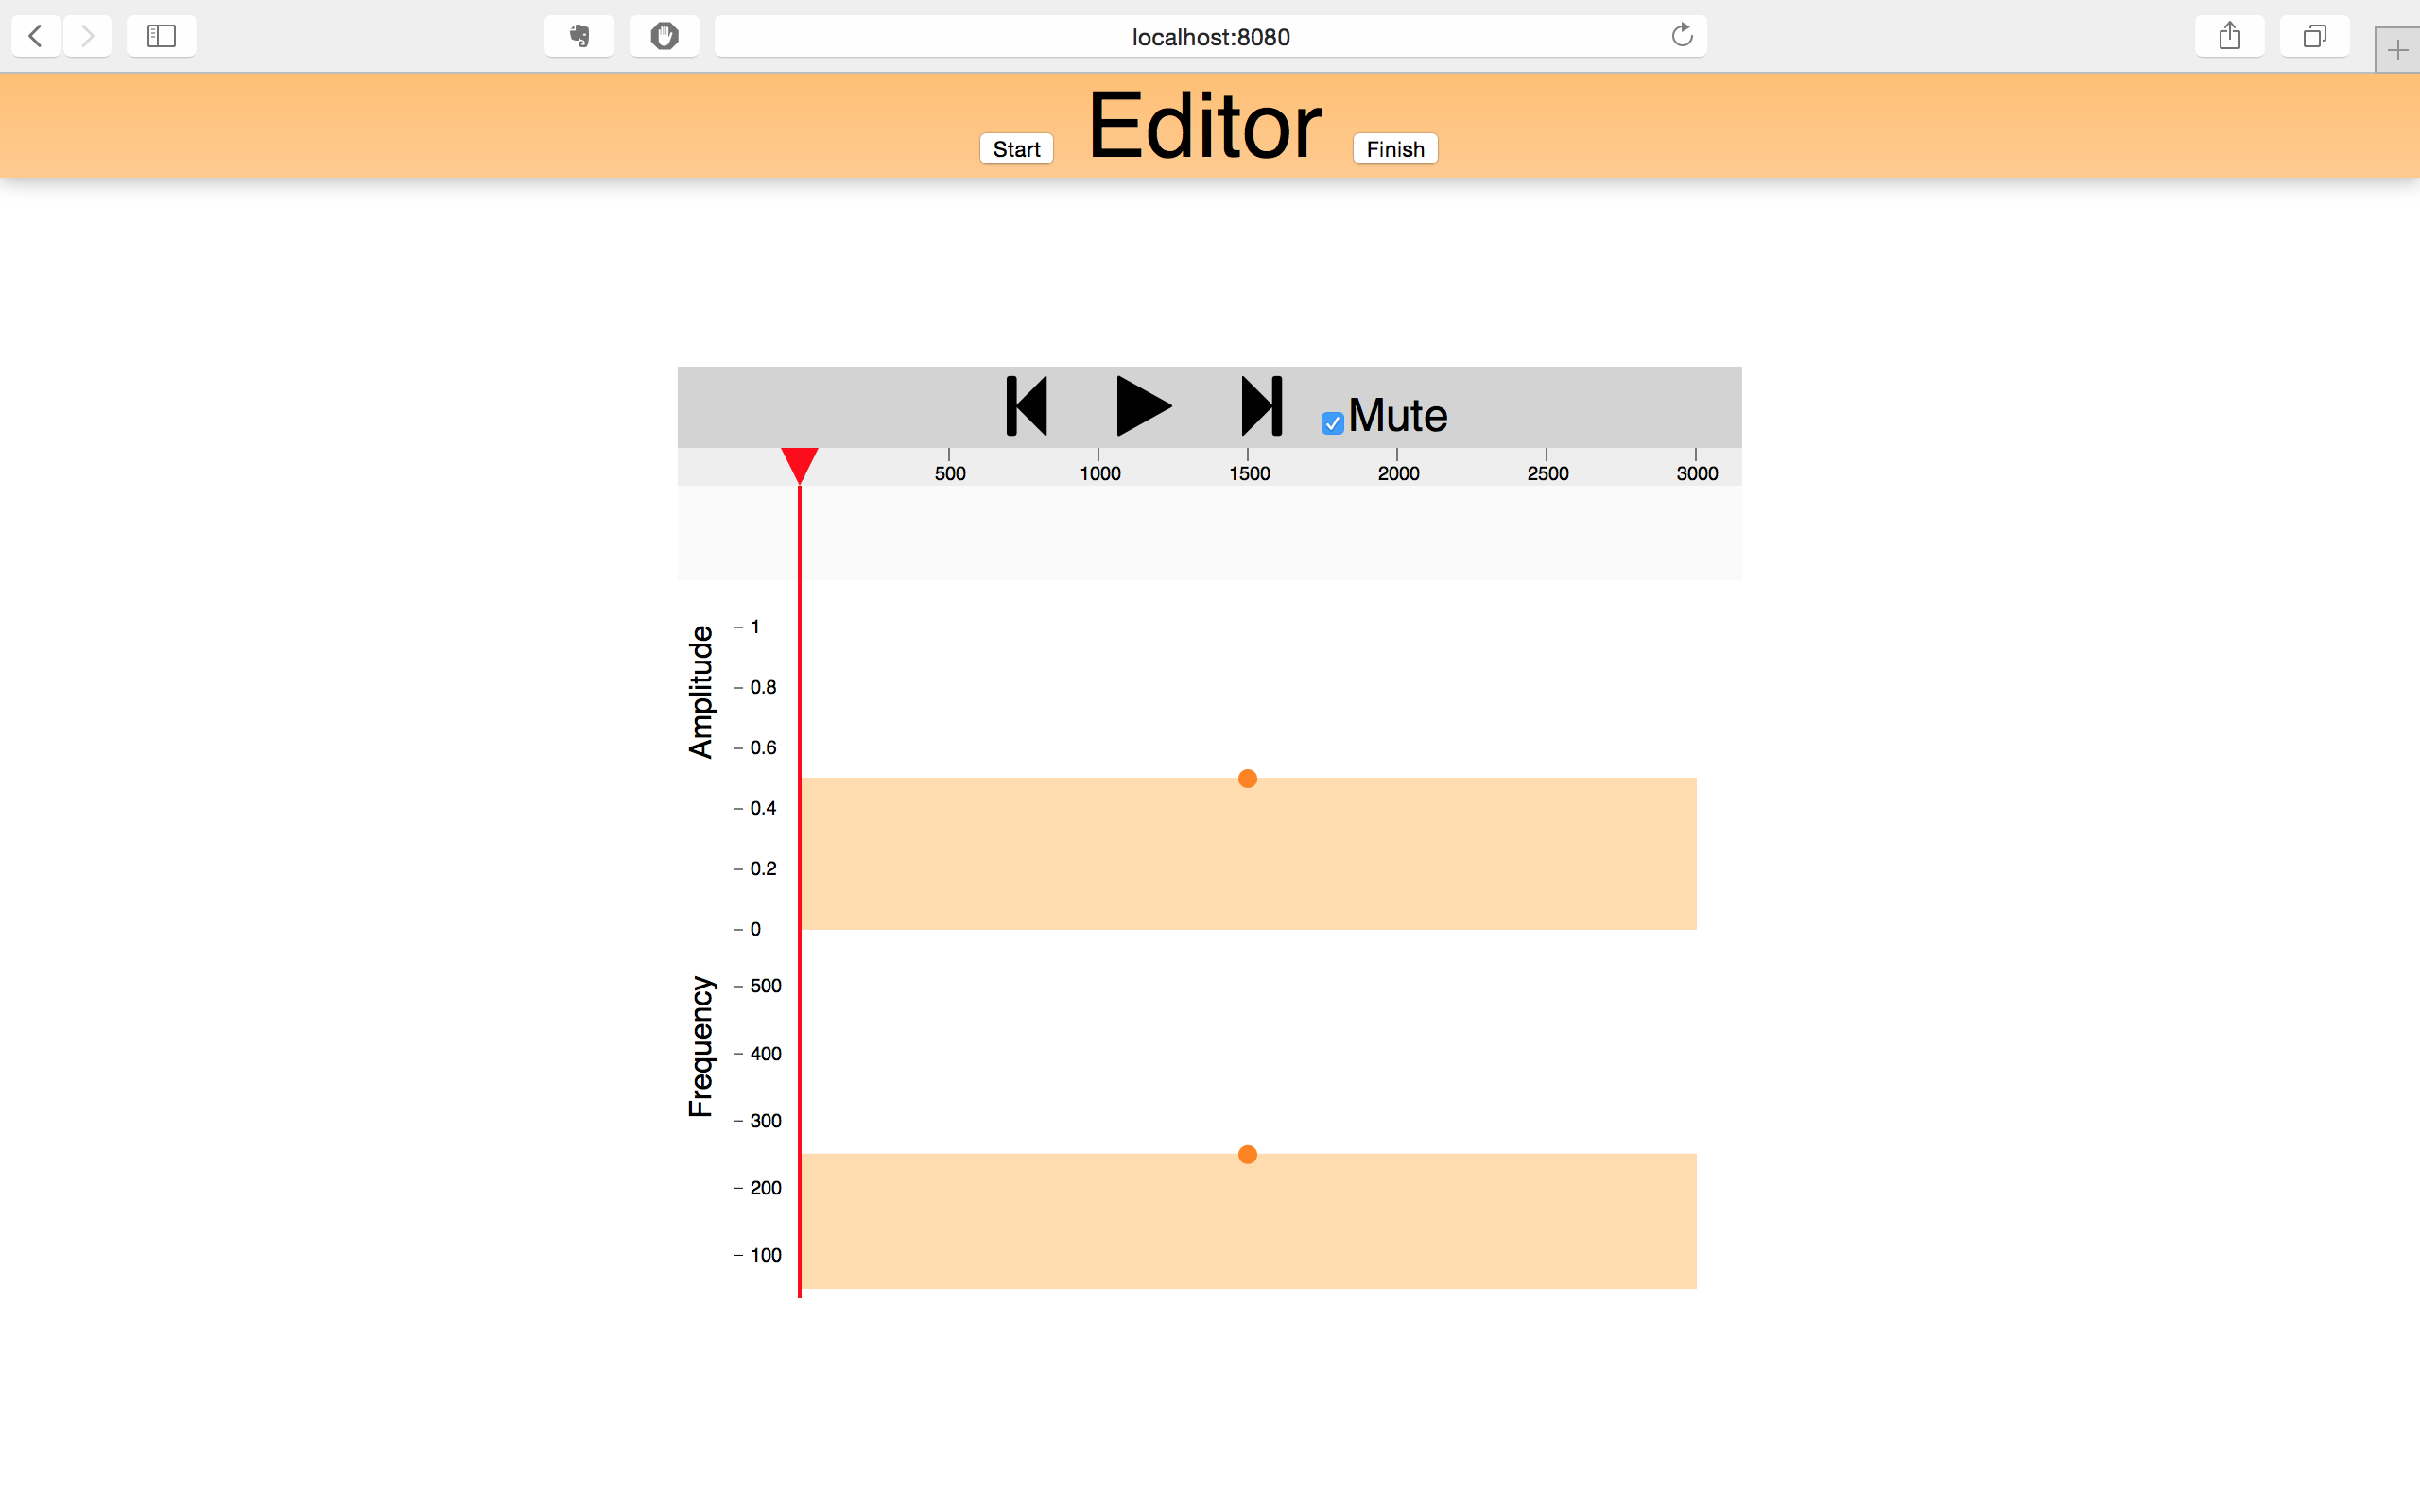
\includegraphics[width=\textwidth]{MacaronScreenshotNone}
%     	   \caption{\none version.}
%     	   \label{fig:macaron:none}
%         \end{subfigure}
    
%     \caption{Alternative Macaron interfaces. \lo has examples that can be felt, but only the waveform is visible (simulating the status quo for libraries). \select shows the vibration, and allows selection and copying from the waveform visualization. \vis is the opposite: showing the underlying vibrations, but with no selection or copying. \none has no examples at all.}
%     \label{fig:macaron}
% \end{figure*}


%%%%%%%%%%%%%%%%%%%%%
%
% SECTION: Related work
%
%%%%%%%%%%%%%%%%%%%%%
\section{Related Work}
% Previous work includes VT effects, past approaches to VT design, and example use in non-haptic design.

%%%%%%%%%%%%%%%%%%%%%%%
\subsection{Salient factors in VT effect perception and control}
% Haptic icons  have long been an important tool for structuring vibrotactile design, typically manipulated with amplitude, frequency and waveform~\cite{Gunther2002,MacLean2003,Brewster2004,maclean2008foundations}.
Vibrotactile effects (e.g. haptic icons~\cite{MacLean2003}) are typically manipulated with low-level engineering of signal parameters, beginning with  amplitude, frequency and waveform~\cite{Gunther2002,MacLean2003,Brewster2004,maclean2008foundations}.
%
%Different granularities of amplitude and frequency control show that
Rhythm can support large, learnable icon sets \cite{Ternes2008,Swerdfeger2009a};  combining waveforms enhances roughness \cite{GunhyukPark2011}.
Time-varying amplitude adds musical expressivity, from tactile crescendos \cite{Brown2006} to 
%attack-decay-sustain-release (ADSR)
envelopes \cite{Schneider2014}.
Multi-dimensional scaling % (MDS)
can be used to identify %, confirm, 
and elaborate these parameters \cite{MacLean2003,VanErp2003,Enriquez2006,Hollins2000}.

Affect and metaphor are another way to structure and manipulate sensations at a level more cognitively relevant than engineering parameters.
Perceived valence (pleasantness) and arousal can be influenced by  frequency/amplitude combination \cite{YongjaeYoo2015,Obrist2015}.
Metaphors \cite{chan2008,Obrist2013,Seifi2015} and use cases \cite{chan2008,Seifi2015} offer structure, memorability and design language.
% While we focus here on single-actuator displays, 
Spatial displays require additional controls for location and direction, % for users to work with, 
whether body-scale \cite{Gunther2002,Israr2011a}, mobile  \cite{Seo2013}, or mid-air \cite{Obrist2015}.
While many parameters are available for VT design, we chose the most established (time-varying frequency and amplitude) for Macaron's initial implementation.
%Location and direction also influence affective perception \cite{Obrist2015}.
%\kmC{summarize? slc} % KM 11.07 1143 this section needs a brief capture statement. My rework of ss heading helps, but problem is,  you've listed a ton of parameters, but not said how this relates to Macaron. This would be a place to say "we chose the three most basic ones to start exploring these ideas (freq, amp, time invariance), but clearly there's a lot of headroom to bring in other manipulables in the future?

%\begin{itemize}

%\item (briefly) what parameters today's technology gives control discretion over, and the scale at which these play out (temporal granularity? thinking about difference between amplitude and rhythm). Mention technology insofar as to say ``this is what the tech requires you to control; and this is what people perceive as perceptual dimensions that thus should be controlled''.

%\item what parameters have been found to have expressive benefit (rhythm wins, waveform loses). Emotional parameters (Sri, Seifi)


%\item what expressive control entails. Focus here on the stimulus properties and their perception, not the tools used to draw them out.

%\item while design space is certainly more limited than visual and auditory design, a considerable and expressive freedom exists (e.g. Ternes, Swerdfeger thesis - pretty large sets are learnable). 

%\osC{missing some synthesis, slc} %KM: I haven't been able to fully process or express what you've suggested here
%\item what makes it hard to access the expressivity that does exist is: 
%(a) serial nature that can be hard for an editor to represent in overview and in comparison with alternatives (a challenge faced by other temporal-media editors) 
%(b) poor predictability of how superposed dimensions (e.g. tracks) will interact perceptually (?)
%(c) big problem: machine parameters aren't necessarily the right perceptual parameters [but, this isn't quite the one you're going after here] 

%(d) ``blank sheet'' problem - perennially needing to start from scratch - identify as the one you're focusing on here.


%\end{itemize}


%\noindent Fodder: 

%- Amplitude and frequency are identified as the primary low-level design parameters for single-location VT actuators \cite{Gunther2002,Schneider2014}.
 
 %- rhythm and other time-invariant patterns occur at a different scale; perceptually extremely important -  Mention van Erp 2003, Brown 2006, Ternes 2008

%- Waveform less expressive \cite{Gunther2002}.

%%%%%%%%%%%%%%%%%%%%%%%
\subsection{Past approaches to VT design}
% Several tools have been built to aid VT design.
Past editors -- e.g., the Hapticon Editor \cite{Enriquez2003}, Haptic Icon Prototyper \cite{Swindells2006}, posVibEditor \cite{Ryu2008}, Vivitouch Studio \cite{Swindells2014}, and Haptic Studio (www.immersion.com) -- are track-based, with graphical representations to edit either waveforms or profiles of dynamic parameters.
Additional features (e.g., spatial control or mobile interfaces) are surveyed in \cite{Schneider2015}.
%Features include the combination or multi-tracking of effects, utilizing a library of existing effects, and the ability to play back sensations.

A library of effects is critical for haptic design tools \cite{Schneider2015}. Most existing tools support feature saving/loading, and some have an internal component library \cite{Enriquez2003,Swindells2006,Swindells2014}.
However, previous implementations were primarily \emph{compositional}, employing building blocks~\cite{Enriquez2006} %that can be combined to create more complex sensations \cite{Enriquez2006}.
rather than complete artifacts. Example use was not studied.
%In Macaron, we also investigate examples of full, created and complete artifacts, built right into the tool.
%\kmC{careful/confused slc} 
% in this par you seem to be saying existing libraries only have bits, not full things. [caution: Swindells examples allowed for examples to be complete as well as partial. I'd back off on this.]
% in next par, you seem to say the opposite: libraries only have whole examples, you can't pick and choose from internals. 

%This  \kmC{what is??} is more analogous to 
% Complete artifacts are found in large libraries of VT icons, but with limitations.
Large VT libraries contain complete artifacts, but impose a serious constraint on their use.
In the Immersion Touch Effects Studio library,
% of tactile icons supplied on a mobile platform, but 
underlying structure and design parameters are hidden and cannot be incorporated into new designs. %, and examples cannot be incorporated into a new project.
VibViz \cite{Seifi2015} features 120 VT examples with visualizations searchable by several taxonomies, but the selection model is all-or-nothing.
FeelCraft \cite{SchneiderAsiaHaptics2014} proposes a community-driven library of feel effects \cite{Israr2014} for simple parametric customization and re-use. %\kmC{and?} % how does Feelcraft fit in here? are you talking about FC in next sentence? if so, need to connect end-user customization better to FC.
While end user customization-by-selection is important \cite{Seifi2014},  
experts need a more open, editable model,
% we suggest a more open model for experts. %this \kmC{what?} still represents a library of selectable, all-or-nothing designs.
%Compare this to
% For example, web designers can view source code at any time, with recent tools allowing search and easy incorporation of elements
just as web designers rely on full access to source code with recent tools allowing search and easy incorporation % of elements
% interactive \emph{design galleries} allow users to search and incorporate elements from other sites 
\cite{Lee2010a}.
% search sites to see what others are doing \cite{Lee2010a}.
%\kmC{Needs summary sentence to close slc} % KM 11.07 1140 this section needs a focus - I'm uncertain of the point being made with the cited work, they seem contradictory. In addition to comments above, suggest close with a sentence on "hole left that this work fills". 
% ALSO, this section seems a little long >.25/6 pgs+ 8-10 refs - although it is likely most impt part of RW, consider dropping one or two cases.

% \begin{itemize}
% \item Other editors have had some success in going after "what makes VT design hard''. They've introduced track-based design, exposed underlying parameters, helped with rapid prototyping, visualization, and sharing of sensations. They vary in the degree to which they support``choosing'' vs ``modifying'' (use Seifi terminology) and how they expose innards. 

% \item Past use of examples goes this far: Swindells allows things to be saved and re-used (but not sampled, and only used in narrow ways), VibViz allows library browsing but doesn't show underlying construction (well, a bit). Immersion editor...

% \item Here, we aren't so much introducing new features or abilities, but we want to turn the knob on the ``example'' thing to see how it actually impacts the design process.  [i.e., don't claim that Macaron is first to employ examples. But do say that it is novel to study it in a variable way]

% \end{itemize}


%%%%%%%%%%%%%%%%%%%%%%
\subsection{Examples in non-haptic design}
% [actually, suggest leaving this out. Already said in 1st para.] Innovative recombination of existing ideas is at the heart of many design inventions~\cite{Warr2005}, and is spurred by immersion in an example-rich environment \kmC{REF?}.
%Creative tasks, like design, are often defined as the recombination of existing ideas, with a twist of novelty or spark of innovation by the individual creator \cite{Warr2005}.

Problem preparation -- also known as the ``problem setting" \cite{Schon1982} or ``analysis of problem"~\cite{Warr2005}
%\osC{or ``collect"~\cite{Shneiderman2000}} 
step of design -- involves 
% getting a handle on the problem 
immersion in the challenge
and drawing inspiration from previous work. %, and and establishing a first general approach with which to attempt a solution.
%Sch\"{o}n demonstrated that designers initially frame their problems before developing a solution \cite{Schon1982}.
%Sch\"{o}n also describes the designer's repertoire, their collected experience, which aids in design.
Both may come from the designer's experience,  \emph{repertoire}~\cite{Schon1982} or exposure to a symbolic domain, e.g., mathematical theorems and notation %, or techniques for painting
\cite{Csikszentmihalyi1996}.

To this end, external examples are critical in inspiring, guiding and informing design \cite{Herring2009,Buxton2007}. 
Industrial designers collect objects %various knobs
and materials; web designers bookmark sites \cite{Herring2009}.
In graphics and web design, \emph{design galleries} organize examples to be  immediately at hand % in the design process
~\cite{Lee2010a,Marks1997}.
% \emph{Design galleries}  are used in graphics and web design to include examples immediately at hand in the design process~\cite{Lee2010a,Marks1997}.
Example-based tools often use sophisticated techniques to mix and match styles and content~\cite{Kumar2011}: this requires immediate access to the examples' underlying structure.
% , requiring access to examples' underlying structure.
%

%%%%%%%%%%%%%%%%%%%%%
%
% SECTION: System Design
%
%%%%%%%%%%%%%%%%%%%%%
\section{Apparatus Design}
%\kmC{OS *slc*}
% KM 02.02: (1) HEADINGS. the submitted-version headings reinforce a "build system / evaluate it" contribution model that may be leading reviewers to overlook the other contributions here. Think about tweaking the names to emphasize the scientific contribution? 
% (2) NOVELTY: this first paragraph of 'system design' is very important in establishing the objectives of the system, and also its novelty. I've tried tweaking it to push forward its experiment-driven requirements. But no novelty as a tool is expressed in this para. We have to either/both of explaining that achieving the flexibility (for an experimental platform) was hard, or that something about the tool itself is novel (and hard). Otherwise, it does sound ho-hum. Obviously this includes example use (shows up in 2nd para, I'll try to work it into first), but can we express something concrete about the rest?
%
To investigate VT design in the context of examples, we required a platform that would expose users' natural procedural tendencies. 
Our Macaron design gallery is simple, flexible, and extensible.
In this work, we add multiple types of example access to polished implementations of familiar concepts: \emph{tracks}, \emph{envelopes}, and \emph{keyframes}
(Figures~\ref{fig:macaron:hi},\ref{fig:versions}).

\begin{figure}[htb]
    \centering
    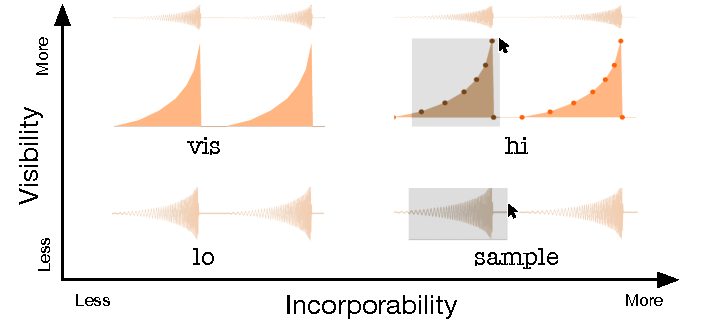
\includegraphics[width=0.75\textwidth]{VersionSpace-16-01-29}
    \caption{Design space for Macaron versions. \hi and \select both allow for selection and copying of example keyframes. \vis and \hi both show the underlying profiles. \lo represents the current status quo; only a waveform is shown.
    %\osC{slc}%"extraction/extractability"? ``sample-ability''?
    %\kmC{slc} % 11.07 10:40 I'm getting weird shadowing in this one, pretty sure it's not right. If it is, I don't understand what I'm seeing. Also it's a big figure and may not be pulling its weight.
    %OS: 02.01 I've adjusted contrast and shading issues. Does this look better?
    }
    \label{fig:versions}
\end{figure}

\begin{table}[htb]
            \small
            \centering
            \begin{tabular}{p{0.5in}p{4in}}
%            \toprule
             \textbf{\hi} & 
                  Full access to gallery examples, with keyframes visible and selectable for copy and paste.
                Simulates source visibility, \emph{e.g.}, viewing the source of a web page or having access to a {\tt .psd} PhotoShop document.
    	        \\
    	    \midrule

    	    
    	    \textbf{\select} & 
                Hides underlying parameters of frequency and amplitude, whereas waveform regions (underlying keyframes) may be copied and pasted into a design,
                simulating example mixing in absence of visibility into underlying construction.
                While possible to see underlying representation by copying the entire example, the steps are indirect and inconvenient.
             \\
    	    \midrule
    	    
    	    \textbf{\vis} & 
                Reveals underlying parameters, but hides keyframes, parameter scales, selection and copy/paste features.
                The inverse of \select, it exposes example structure, but does not support incorporating example elements into a design.
             \\
    	    \midrule
    	   
    	        	    
             \textbf{\lo} & 
                Supplies a ``black box'' outer representation. Playback and visualization of the complete vibration reflect the status quo of non-visible, non-mixable example libraries.
             \\
    	    \midrule
	    \textbf{\none} & 
                No examples present.
             \\
%             \bottomrule

    	    
            \end{tabular}
            \caption{Macaron tool alternatives, varied on dimensions of internal visibility and element incorporability.}
            \label{tab:toolAlternatives}
        \end{table}
  

\emph{Tracks} are the accepted language of temporal media editors (video, audio, and past haptic efforts \cite{Swindells2006,Enriquez2003,Ryu2008}).
We provide tracks for perceptually important ``textural'' parameters (amplitude and frequency); the user accesses periodic and time-variant aspects by manipulating their 
\emph{envelopes} using
%Effects are further encapsulated as 
\emph{keyframes}, with linear interpolation in-between.
Users double-click to create a new keyframe, click or drag a box to select, and change or delete a selection by dragging or with the keyboard.
A waveform visualization reflects changes.

Macaron's example access features are inspired by more recent graphics and web design galleries \cite{Marks1997,Lee2010a,Ritchie2011}, which show examples side-by-side with the editor.
% to help ground the designer.
Other implemented features, critical for polished creative control \cite{Schneider2015}, include real-time playback, time control (scrubbing) % by the red play-bar, 
copy-and-paste, undo and redo, and muting (disables realtime VT output).
% Users can mute vibration output. 
%
To support its use as an experimental tool, user interactions are logged; 
start / stop buttons allow the user to indicate when they began and completed their design process.

 
Macaron was built with HTML5 and JavaScript, using React, Reflux, D3, and
Audiolet\footnote{\url{facebook.github.io/react}, \url{github.com/reflux}, \url{d3js.org}, \url{github.com/oampo/Audiolet}}. Real-time sound synthesis drove a C2 actuator.
To leave % the user's 
hands free for keyboard and mouse, the C2 is attached to a wristband; we simulate the design process for a wrist-worn wearable (as in \cite{Seifi2015}).


%
% Subsection: Alternative Versions
%

%\subsection{Alternative Versions}
%\kmC{descriptive version names?}
\emph{Evaluation Versions}: To study how examples impact design, we made four gallery versions by sampling two theoretical dimensions of example access:
% example visibility and incorporability (\autoref{fig:versions}).
element \emph{incorporability} and internal parameter \emph{visibility} (\autoref{fig:versions}, \autoref{tab:toolAlternatives}).
We hypothesized these would affect users' design processes, e.g., incorporable examples would encourage ``mixing and matching" of examples, visibility might provide insight.
%\kmC{OS: slc} % reads very oddly to have this results-type sentence here. Recall a discussion, can't remember reasoning. Can we drop it?
%However, these different versions revealed that our participants used these examples in a more nuanced way: as a \emph{starting point for each design}, and \emph{scaffolding for learning}.
%Our results indicated this nuanced.
%, two of which are analogous but not identical to visibility and incorporability.
%We discuss this later. %  finding not quite lining up with these dimensions.
%We theorize that the first, which opens the ``black box'' that is closed in most example libraries, will assist learning, encourage deconstruction, and promote internally intensive strategies like superposition (e.g., modifying envelopes of individual tracks as opposed to just pasting together frames sequentially). 
%Incorporability, on the other hand, should promote re-usability and efficiency, but it might not necessarily improve learning or sophisticated editing methods.

We compared these versions with each other and with a non-example version:
\none.
%
%\hi (\autoref{fig:macaron:hi}),
%\lo (\ref{fig:macaron:lo}),
%\select (\ref{fig:macaron:select}),
%\vis (\ref{fig:macaron:vis}).
%
In all versions with examples, the user can play or scrub the example, feeling it and seeing the waveform visualization.
We did not allow users to modify the examples, to avoid study workflow confounds.
To populate the gallery, we chose or adapted seven examples from~\cite{Seifi2015}, 
piloted them to confirm example variety, then regenerated keyframed versions with Macaron.
% To populate the gallery, seven examples were chosen or inspired from~\cite{Seifi2015}, piloted to confirm example variety, then keyframed versions were re-generated with Macaron.




%%%%%%%%%%%%%%%%%%%%%
%
% SECTION: Study
%
%%%%%%%%%%%%%%%%%%%%%
\section{Study Methods}
% \section{Study Method}
%\kmC{slc} % OS, I don't like my new section title much. Can you do better? I want to allude to what the study is about, to avoid natural assumption it's for tool usability.
Participants were tasked with creating a sensation to accompany five animations (\autoref{fig:animation}) -- SVGs (scalable vector graphics)  which can be played or scrubbed by the same means as navigating Macaron's time control.
We chose animation variety (concrete to abstract) and complexity to inspire non-obvious solutions without overwhelming.

Participants were first trained on \none\ with no animation,
then presented with five animation/version combinations.
As the least crucial source of variance, animations were presented in \autoref{fig:animation}'s constant order, while 
interface versions were counterbalanced in two 5x5 Latin square designs.
Thus, each participant encountered each animation and each interface version once; over all participants, each animation/version combination appeared twice,
with Latin squares balancing 1st-order carry-over effects.
This design confounds learning with animation task. 
We believe this is an acceptable tradeoff at this stage, allowing us balance interface order with a single participant session of reasonable length (1-1.5h).
% Once we understand the effect of example interfaces, we can choose a single version and examine other factors in future work.


% I come out of this feeling confused about factors and rationale.
% - explicitly state the factors you KEPT (incorporability and visibility) and the one you dropped.  
% - Why can you afford to overlook learning?
% - define what you got, for the price of the confound: be explicit about the constraint being satisfied.  there is both fitting a session into a single subject's time, and not choosing to run more subjects to keep the design iteration lightweight in proportion to the investigative stage. 

\newcommand{\animationHeight}{0.75in}
 \newcommand{\animationWidth}{0.27\textwidth}
%\newcommand{\animationWidth}{0.095\textwidth}

\begin{figure}[htb]
    \small
    \centering
    \begin{subfigure}{0.18\textwidth}
            \centering
            
\includegraphics[height=\animationHeight]{animations/MacaronHeart}
    	   \caption{Heartbeat.}
    	   \label{fig:animation:heartbeat}
    \end{subfigure}
    \begin{subfigure}{0.18\textwidth}
            \centering
            
\includegraphics[height=\animationHeight]{animations/OliverCat}
    	   \caption{Cat.}
    	   \label{fig:animation:cat}
    \end{subfigure}
    \begin{subfigure}{0.18\textwidth}
            \centering
            
\includegraphics[height=\animationHeight]{animations/OliverLightning}
    	   \caption{Lightning.}
    	   \label{fig:animation:lightning}
    \end{subfigure}
    \begin{subfigure}{0.18\textwidth}
            \centering
            
\includegraphics[height=\animationHeight]{animations/OliverCar}
    	   \caption{Car.}
    	   \label{fig:animation:car}
    \end{subfigure}
    \begin{subfigure}{0.18\textwidth}
            \centering
            
\includegraphics[height=\animationHeight]{animations/MacaronSnow}
    	   \caption{Snow.}
    	   \label{fig:animation:snow}
    \end{subfigure}
    
    \caption{Animations used as design tasks, in presentation order. Heartbeat expands in two beats; the cat's back expands as breathing and purring; lightning has two arhythmic bolts; the car oscillates up and down, and makes two turns: left then right; snow has three snowflakes float down.
    %See accompanying video for more detail.
    }
    \label{fig:animation}
\end{figure}



\section{Results}
 
% 1. earlier you called them "designers" - might require qualification.
%
% 2. Later you mix in "I" with "P" subjects. I think (not sure) that you ran 13 subjects, but discarded 3 incompletes. This is a confusing way to say it; when you first identify the incompletes, along with P9, I can't tell what's what. Is it P1-P10 plus I1-I3? Indicate this right here where you identify subjects.
%
% 3. Better justify N=10. Later, it gets awkward when you note you only have 2 observations each. We know people will ask for more data; I don't think what's here is strong enough to counter. Need to indicate the COST of running a subject? relative to benefit? 20 would not be an unusual number for a psychophysics experiment. The point here is the analysis is hell. 

We targeted a study size of 10 complete participants for a balanced Latin square design, and a manageable sample size for rich, exploratory, qualitative analysis. % for an exploratory investigation.
13 untrained  participants were recruited: P1-10  (7 female, ages 22-35) completed all five tasks, while I1-3 (2 female, ages 29-45) 
% did not complete all designs due to time restrictions,  
only completed the first three % (heartbeat, cat, lightning) 
due to time restrictions.
% This may be due
Because I1-3 (and P9) all had the same interface order (\lo, \none, \vis, \hi, \select), we suspect that beginning with `sparse' versions gave insufficient insight into how to design quickly enough to finish the study. % into how to use examples.
I1-3 showed no distinct patterns beyond this; we leave their data for future analysis.  
%when we can follow-up with additional studies. 
% other than time constraints to not finish the study.
% After I1-3 failed to complete this order, P9 did complete it.
 
%


% We outline these, then describe the two main ways we saw examples used: 
% \kmC{SLC} % Note, this statement is repeated at start of (C) example use. I wonder if it would be better to give this preview in the Intro, but leave it out here?
% directly within each task as \emph{design starting points}, and indirectly over the session to \emph{learn how} to make VT designs.

\emph{Analysis and Data:} A team member % OS, should this be "team member?"
trained in qualitative methods analyzed screen recordings, interviews, and logs with grounded theory methods (memoing, open \& closed coding~\cite{Corbin2008}) and thematic analysis and clustering \cite{Moustakas1994}.
We visualized logs using D3 (\autoref{fig:archetype}). 
%
We chose a qualitative analysis because our goal was to capture the design process, not compare Macaron with previous tools.
% Qualitative analysis was chosen to capture the design process, rather than comparison with previous tools.
Our analysis exposed three major qualitative findings, discussed below.
%We now discuss our three major qualitative findings: 
% an archetypal process followed by participants, individual micro-interaction patterns, and strategies for example use.

%
%\kmC{slc} % I'm trying sticking this part about participants under "analysis", rather than as part of what looks like a usability comment. I believe you're not attributing the noncompletion to a lack of tool usability, but rather to task comprehension. But generally, the following statements are confusing and need to make a point more clearly.
%For each condition, participants were able to complete all 5 designs within their sessions, \kmC{[?? slc]  
%with one exception: three participants ran out of time, failing to finish all of P9's condition before P9 finally did.}
% P9 is one participant not 3. What does it mean that 3 (out of 10, this is not an exception it's a major proportion) failed to finish P9's condition before P9 did?  And how do the I1-3's count re latin square? 


\emph{Tool Usability:} Overall, the tool was well received, described as \qquote{P1}{easy to use}, \qquote{P5}{well made}, %\qquote{P7}{cool}, %\qquote{P7}{awesome},
\qquote{P9}{pretty neat}, \qquote{P3}{the templates help a lot}.
%\kmC{any more reserved comments to balance these, or more detailed insights about usability relevant?}


\emph{Completion time:}
%While we asked participants to click the ``start" button before they started designing, some clicked before browsing examples, and some afterwards.
%Therefore, w
%We calculated task time from handing off the mouse to the participant to the user's hitting the ``finish" button. %\kmE{located XX}.
Overall mean task completion time for P1-10 was 5m48s (median 4m48s, sd 3m52s, min 40s, max 18m23s).
%With two observations for each interface/task combination, 
We conducted two one-way ANOVAs on  completion time;
%,  with interface or task as factors.
%; diagnostics of normality (S-W test failed, but it's equal sample size and QQ plots showed limited violations. Also, Kruskal-wallis test corroborated ANOVA results) and homoscedascity (Levene's test) both passed.
%INTERFACE:(Shapiro-Wilk failed W=0.92, p=0.00192, but inspectino of QQ plots revealed limited skewness; Levene's test
%INTERFACE LEVENE TEST F(5, 44) = 0.8428 p=0.5268 
%INTERFACE ANOVA: $F(5, 44)=0.3596$ $p=0.8733$
%TASK S-W: W = 0.94902, p-value = 0.0311
%TASK LEVENe F(4, 45)=1.4966 p=0.2192
%TASK 
neither interface ($p=0.87$) nor task ($p=0.64$) had a significant effect. % on completion time.


\begin{figure}[tb]
    \centering  
    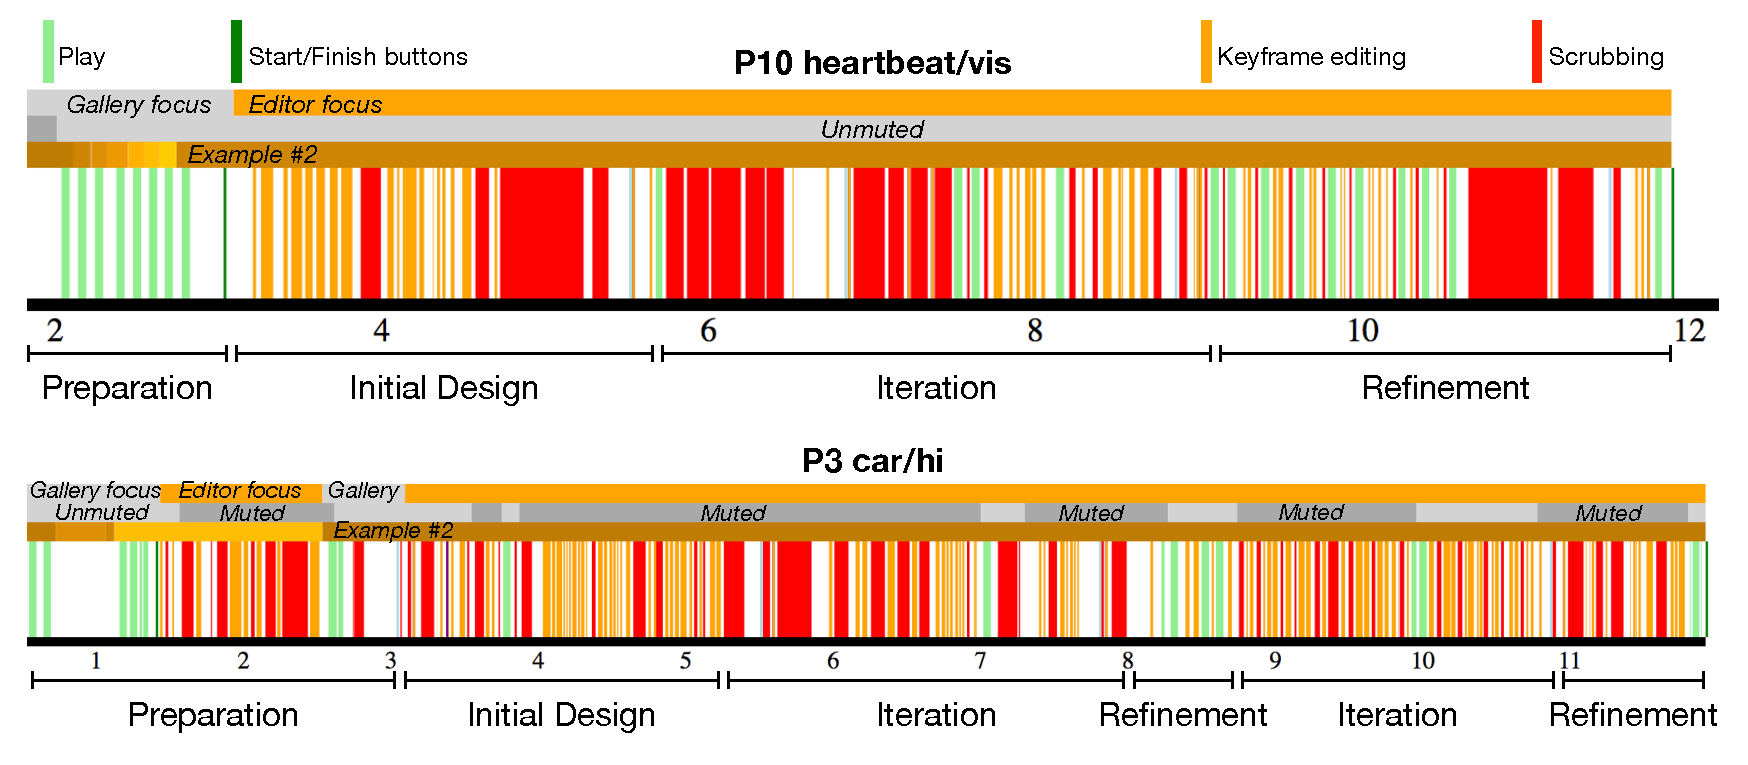
\includegraphics[width=\textwidth]{timelines/Example-Process-Diagram4}
    \caption{Log visualizations showing archetypal design process. Top: P10's heartbeat/\vis condition (an``ideal'' version). Bottom: P3's car/\hi condition (variations: a return to example browsing after editing, repeated refinement, muted editing).
    } 
    \label{fig:archetype}
\end{figure}


\begin{table*}[]
	\small
            \centering
            \begin{tabular}{p{0.5in}p{4in}}
%            \toprule
             \textbf{Prepare} & 
                All participants began with a problem preparation step \cite{Warr2005}. They played the animation to understand the problem, then typically looked at several (sometimes all) examples.
                %All participants browsed browsed at least one example once; 
                Only P2, P8, and P9 had a task where they did not begin with an example.
                Otherwise, participants browsed examples, chose a best match to the animation (\qquote{P7, heartbeat/\hi}{I was trying to find the best match with the visual}), then transferred into initial design. 
                Participants rarely returned to examples for more exploration; only P3 (car/\hi) and P5 (car/\lo) switched to a different example after beginning their initial design.
                Preparation is characterized by a large number of plays and example switches: on average, 47.45\% of all session plays were before the first edit (sd 30.15\%),
                %(todo- remove cases where I played),
                and participants switched examples an average of 6.75 times (sd 5.17).
             \\
    	    \midrule
    	    
             \textbf{Initial Design} & 
                Participants either used their example choice to help create their initial design, or ignored it because it wasn't close enough to what they wanted to do.
%                \kmC{SLC x2} 
                % 1. "what they wanted to do" suggests a vision that is apart from the example inspiration. Talk about that?
                % 2. In below: I'm so uncertain about what the gallery versions are (nondescriptive names) that it's hard to get import of the details reported. 
                Participants typically recreated the example in their editor by copy/paste of the entire design (P1,2,4-8,10) or sometimes a component (P3,10) in incorporable conditions (\hi and \select), or by manually recreating the design (P5,6) or a component (7,10) with \vis.
                In the \lo condition, we only observed P5 somewhat recreating an example.
                %LOW: P3 lightning/low?, P4 inspired
                Occasionally, participants would create a new design loosely based on the example rather than recreating it (P3,4,6-8), when using the \emph{Inspire} example use strategy (described later).
%                \textbf{TODO: Was this typically in Vis? (it was, need to count).}
             \\
    	    \midrule
    	    
    	    \textbf{Iterate} & 
                % After initial design, participants started iterating to develop their design.
                Participants refined designs with longer periods of editing typically book-ended by playing the entire design (discussed as ``real-time feedback"  micro interaction pattern).
            	In some cases, especially when the example was ``close enough", participants skipped iteration (\emph{Adjust} or \emph{Select} example use strategies, described later).
             \\
    	    \midrule
    	    
    	    \textbf{Refine} & 
                Smaller changes forecast design conclusion, e.g.,
            	incremental global changes: constant frequency (P1,2,5,6,10), alignment (P1,3,6), or pulse height adjustment (P1,3,8,10).
            	This step is sometimes visible in activity logs, as most participants (P1,3-10) exhibited more frequent plays of the entire design, and shorter periods of editing/scrubbing.
            	Occasionally, participants repeated larger iterations and refinement (P3 car/\hi, \autoref{fig:archetype}).
             \\
%    	    \bottomrule
            \end{tabular}
            \caption{Steps in observed archetypal design process.
            % \kmC{put Fig XX color codes here?? tiles under step names?}
            % \kmC{02.02: highlight word "example" in table, to show example appearance in process?}
            }
            \label{tab:archetypal:process}
        \end{table*}
        
        
%
% Archetypal Design Process
%
\subsection{Archetypal Design Process}
 % NEW 02.02  [see radical suggestion in next line!] devil's advocate: while I realize we've treated example use separately from design process (section A, B vs C) as I read A and B I start to wonder why they're here if our objective was just to look at examples use. Can you do a bit more to justify this, and perhaps allude to example influence on the design process? and/or, to the design process in (C)?  
 % [radical suggestion] In Table II, examples appear more than they do in the regular text. What if we highlighted every appearance of the word "example" in table II to illustrate this? You'd need an explanation in the caption, to effect we do this to help see where examples show up in the process we observed.
 %
Log visualizations (\autoref{fig:archetype}) show that users could and did employ Macaron for all key design stages: preparation, initial design, iteration, and refinement. %(\autoref{tab:archetypal:process}, 
% implying that it supported these steps.
All participants followed this sequence.
Some omitted one or more steps depending on personal style and strategies for using examples (below). % Verify - only a single step omitted by any one P, and all followed sequence? Earlier version sounded like "they all did the same thing except some did it differently" - seeking more concreteness about divergence.
We list observations of the basic process in \autoref{tab:archetypal:process}, to document behaviour and frame discussion.
% of example use and individual differences.
%\autoref{fig:archetype} shows an exemplar of this process.






%%%%% MOVED INTO TABLE %%%%%%%%
%     \subsubsection{\underline{Preparation}}
%     All participants began with a problem preparation step \cite{Warr2005}. They played the animation to understand the problem, then typically looked at several (sometimes all) examples.
%     %All participants browsed browsed at least one example once; 
%     Only P2, P8, and P9 had a task where they did not begin with an example.
%     Otherwise, participants browsed examples, chose a best match to the animation (\qquote{P7, heartbeat/\hi}{I was trying to find the best match with the visual}), then transferred it into initial design. 
%     Participants rarely returned to examples for more exploration; only P3 (car/\hi) and P5 (car/\lo) switched to a different example after beginning their initial design.
%     Preparation is characterized by a large number of plays and example switches: on average, 46.67\% of all session plays were before the first edit (sd 29.63\%),
%     %(todo- remove cases where I played),
%     7.78 example switches (sd 5.15).
% 	%⁃	TODO: how many unique examples (“examples viewed”??)
% 	%Participant rationale for choosing or browsing examples is discussed in more detail below. %  with direct example use in tasks.
    
%     \subsubsection{\underline{Initial Design}}
%     % After choosing an example,  usually the closest match to the problem domain or intended design, 
%     Participants either used their example choice to help create their initial design, or ignored it because it wasn't close enough to what they wanted to do.
%     \kmC{SLC x2} 
%     % 1. "what they wanted to do" suggests a vision that is apart from the example inspiration. Talk about that?
%     % 2. In below: I'm so uncertain about what the gallery versions are (nondescriptive names) that it's hard to get import of the details reported. 
%     Participants typically recreated the example in their editor by copy/paste of the entire design (P1,2,4-8,10) or sometimes a component (P3,10) in \hi and \select conditions, or by manually recreating the design (P5,6) or a component (7,10) with \vis.
%     In the \lo condition, we only observed P5 somewhat recreating an example.
%     %LOW: P3 lightning/low?, P4 inspired
%     Occasionally, participants would create a new design loosely based on the example rather than recreating it (P3,4,6-8), when using the \emph{Inspire} example use strategy (described later).
%     \textbf{TODO: Was this typically in Vis? (it was, need to count).}
%     %We describe this later under “Direct Example Use - Starting Point” as a spectrum of approaches: “ignore”, “inspire”, “template”, “adjust”, and “select”.

    
%     \subsubsection{\underline{Iteration}}
    
%     % After initial design, participants started iterating to develop their design.
%     Participants refined designs with longer periods of editing, either by itself or with scrubbing interspersed, typically book-ended by playing the entire design.
% 	They took time to \kmC{??: realize each new version of the design before giving them an overview.}
% 	% While the mute feature was rarely used, [KM: but, 3/7 did. That's not rare.} 
% 	P3, P4, and P7 all exhibited focused editing with mute enabled, unmuting for the bookended play sections; others did not use muting.
% 	In some cases, especially when the example was ``close enough", participants skipped iteration (\emph{Adjust} or \emph{Select} example use strategies, described later).

    
%     \subsubsection{\underline{Refinement}}
    
%     Smaller changes forecast design conclusion, e.g.,
% 	incremental global changes: constant frequency (P1,2,5,6,10), alignment (P1,3,6), or pulse height adjustment (P1,3,8,10).
% 	This step is sometimes visible in activity logs, as most participants (P1,3-10) exhibited more frequent plays of the entire design, and shorter periods of editing/scrubbing.
% 	Occasionally, participants would repeat larger iterations and refinement steps (P3 car/\hi), see \autoref{fig:archetype}.
% 	%Some participants skipped refinement(\emph{Select} example use strategy).
    %%%%%% END TABLE MOVED %%%%%%%

\subsection{Micro Interaction Patterns Enabled by Tool} 
Several small-scale  patterns further characterize behaviour within the archetypal process.

%\begin{figure}
%    \centering
%    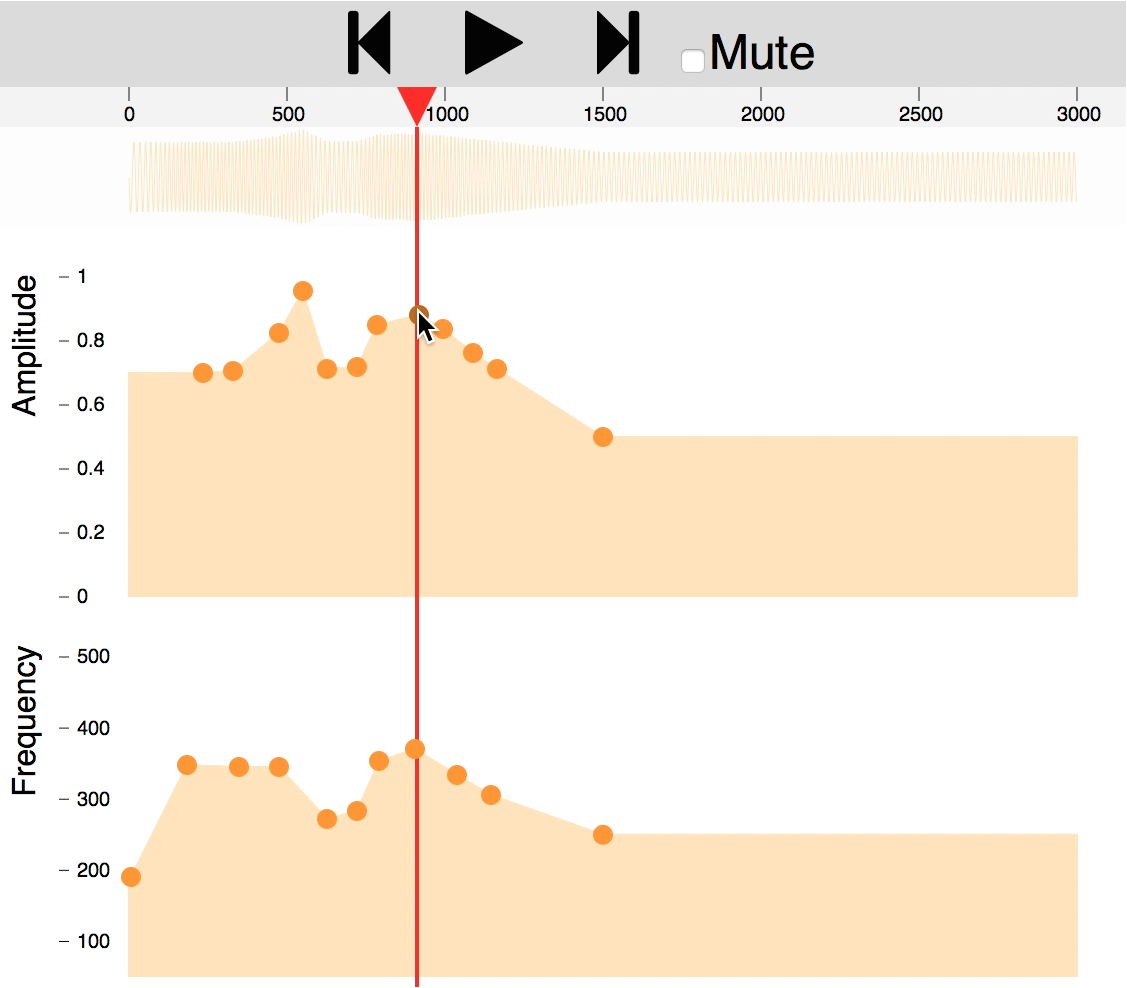
\includegraphics[width=0.24\textwidth]{Alignment-BetweenTracks-P13-Cat-None}
%    \caption{Participants used the red playhead for alignment, between animation and the multiple tracks (P9 cat/\none).
%    \kmC{Drop? slc} % The playhead shows up in other figures, can you reference it there? If so, may need to include the caption}
%    }
%    \label{fig:alignment}
%\end{figure}


\inlineHeading{Different paths through the interface}
% \subsection{Paths through the Interface}
%
% Participants navigated through the interface in different ways.
% We found three strategies that have later implications for design:
% by time, by component, and by track.
% With by time (\autoref{fig:path:bytime}, P1,2,3,4,7,9), participants march through the design, creating amplitude and frequency at the same time.
% With by component (\autoref{fig:path:bycomponent}, P1,4,6,8,10), participants develop and iterate on part of a design, then repeat or copy and paste the component later in time.
% With by track (\autoref{fig:path:bytrack}, P2,3,6,7,8,9,10), participants work through an entire track (typically amplitude) before working through the other one.
% These different strategies are often combined; for example, P6 developed their car/\lo component by track (amplitude, then frequency).
%
%% Further enforcing flexibility, participants frequently used copy and paste to replicate points in time (containing points from one or both tracks), but P1,3,7 also brought up being able to copy and paste between tracks:
%% \qquote{P7}{The one thing I found missing was copy and pasting between amplitude and frequency}.
%    % Participants navigated through the interface in different ways. 
%
%
    We saw three design-path strategies. % that have later implications for design:  %  time,  by component,  and by track.\\
    \par -- \emph{Time} (\autoref{fig:path:bytime};  P1,2,3,4,7,9): proceed through the timeline,  creating  amplitude  and  frequency  at  the  same  time.
    \par -- \emph{Component} (\autoref{fig:path:bycomponent}, P1,4,6,8,10): iterate  on  a  design element,  then  repeat  or  copy/paste it later in time.
    \par -- \emph{Track} (\autoref{fig:path:bytrack},  P2,3,6,7,8-10): proceed through one entire \emph{track} (typically amplitude), then the other one. 
    
 \noindent Strategies were often combined hierarchically. P6 developed a car/\lo component by track (amplitude, then frequency).
    Wanting additional flexibility,   %participants  used copy/paste to replicate points in time (re-using points from one or both tracks),  but 
    P1,3,7  requested  copy/paste  \emph{between}  tracks: \qquote{P7}{The  one  thing  I found missing was copy and pasting between amplitude and frequency}.
 


\begin{figure}[Htb]
\centering
\begin{subfigure}{4.5in}
    \centering
    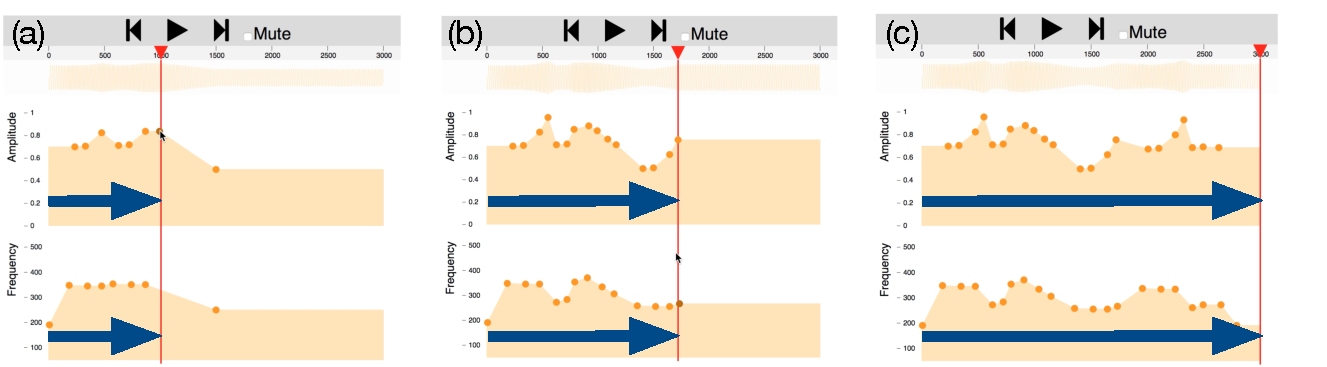
\includegraphics[height=1in]{paths/Path-ByTime}
    \caption{P9's cat/\none design progressed sequentially in time.
    Note the red playhead helping alignment in (b).
     }
    \label{fig:path:bytime}
\end{subfigure}

\begin{subfigure}{3.5in}
    \centering
    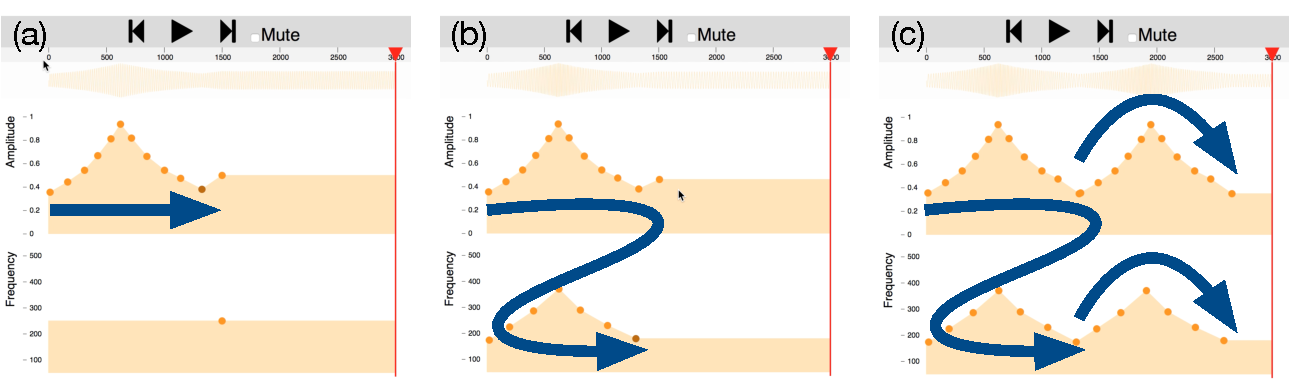
\includegraphics[height=1in]{paths/Path-ByComponent2}
    \caption{P6's car/\lo design progressed by component, developing the component then repeating it.}
    \label{fig:path:bycomponent}
\end{subfigure}

\begin{subfigure}{4.5in}
    \centering
    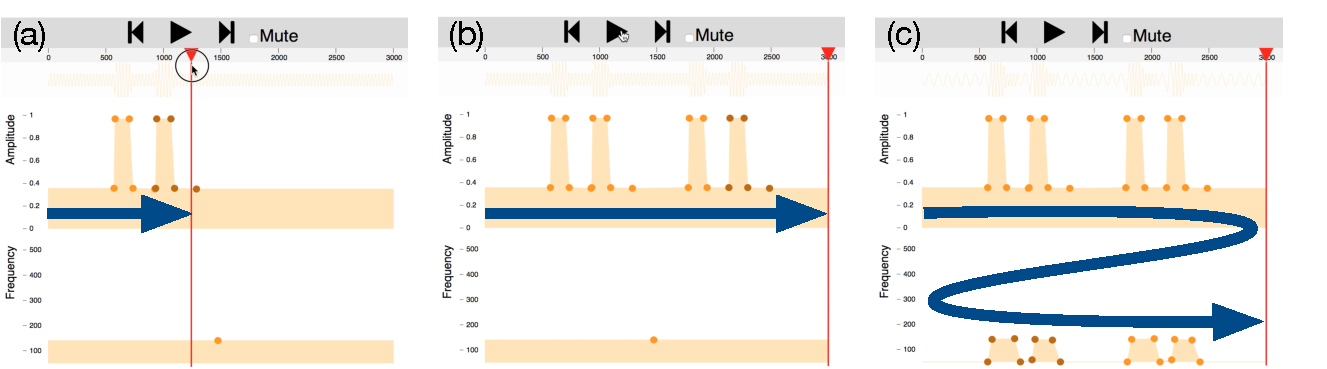
\includegraphics[height=1in]{paths/Path-ByTrack}
    \caption{P10's heartbeat/\vis design progressed by track. Amplitude was developed first, then frequency.
    }
    \label{fig:path:bytrack}
\end{subfigure}
\caption{Participants created their designs using different progression paths, suggesting flexibility.}
\label{fig:path}
\end{figure}
%
   \begin{figure}[Htb]
    \centering
    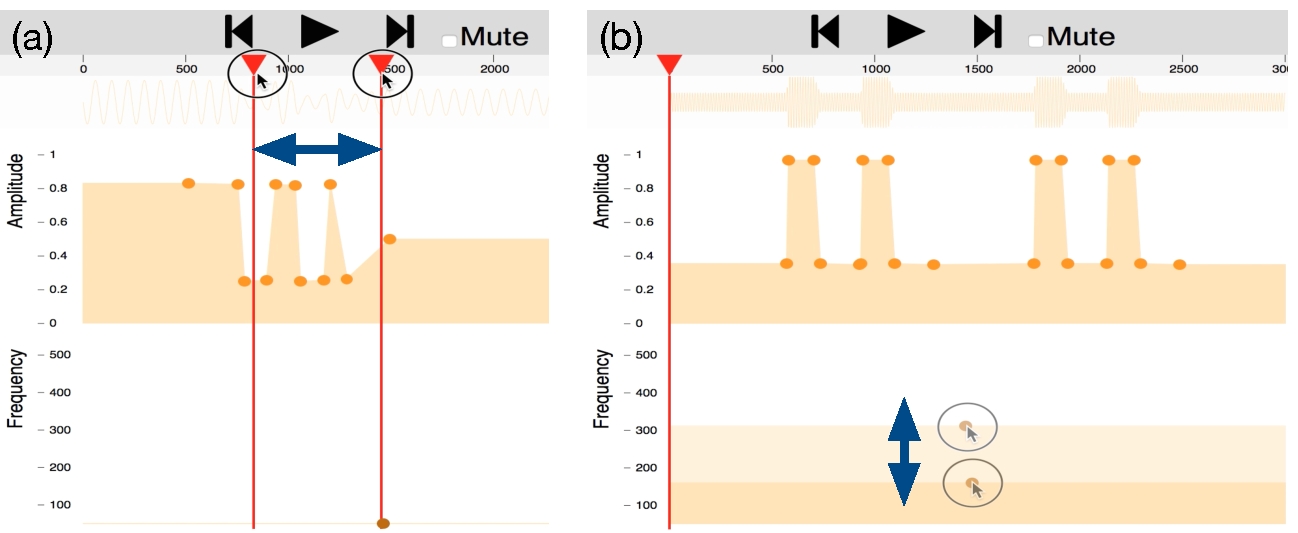
\includegraphics[height=1.75in,width=4in]{realtime/RealTimeFeedback}
    \caption{Participants used real-time feedback to explore, both (a) in time by scrubbing back and forth (P3 lightning/\lo), and (b) by moving keyframes (P10 heartbeat/\vis).
%        \kmC{lose some whitespace? slc.} % do you need the (a), (b) etc in Figs 6, 7, 9? Would get you 3-6 lines of vertical compression.
        }
    \label{fig:realtimefeedback}
\end{figure}
    

%    \kmC{slc} % KM 11.07 1311 Does this par belong under Micro Interactions? clarify why it's a path-thru-interface if not.
    Further showing diverse workflows, participants requested more powerful controls to work with keyframes as a group, such as widen (P5), reverse (P7), shift everything (P9), move up/down and smooth (P4). % these requests  by saying the more power we have, the better: \qquote{P1}{It's always good to have more control over what I can adjust}.
    %This could have an affect on how participants choose their examples or their approach for initial design:
%    \qquote{P7}{None of [the examples] came close...the one I selected was the exact inverse of what I wanted}.
%    \qquote{P7}{The [example] I selected was the exact inverse of what I wanted}.
    Other requested features include looping (P1), hovering over a point to see the value (P1), more detail through a zoomable interface (P4). 
    %OS CUT? P4 discovered and heavily used left/right arrow keys to navigate the timeline, a feature that had not been disclosed but remained in the tool from development.

\inlineHeading{Alignment and Copy/Paste are Precise, Convenient}
%    Participants described both alignment and copy/paste as important features.
    Precision was valued; alignment and copy/paste were used to achieve it.
%       
%       \kmC{is this a novice thing?? SLC} % I wonder if precision desire comes from the tool affordance, and transfer from other editing (visual) where precision can really count. It might be that a precise design is indistinguishable haptically from a nonaligned one, but these subjects don't know that yet.
%       
    Alignment was sought both in time and to keyframe values.
    A common technique (\autoref{fig:path:bytime}b) was to use the red playhead like a plumb-line to align keyframes with animation features (P1-5,7,9,10) and between the two tracks (amplitude and frequency) (P3-5,7,9,10): \qquote{P2}{Using that red arrow thing and placing the dots when it makes the heartbeat}.
    Some participants, including those who used the plumb-line, requested
    %P1,2,6,7,8,9
    %Six participants requested even 
    more refined alignment features: \qquote{P1}{I couldn't keep it straight}. %\textbf{CONFIRM!} \kmC{slc} % Were requestors the same ones who made use of plumbline, or were they ones who hadn't discovered it? i.e. was plubmline enough?
    % Several participants requested alignment features: shift to move in only one of x or y; anchors; alignment of video.

    Copy/paste was used for improved  work efficiency (especially helpful during initial layout or when creating long or repeating designs)
    %\qquote{P1}{If you want to create something that's longer you might want copy and paste},
    %\qquote{P2}{It was easier to use the examples, and it felt like matched, not exactly, but enough}.
%    \qquote{P6}{That was easy, I just copy and pasted the entire thing}.
    and precision:
    \qquote{P6}{Copy and paste...was also the most precise, because if you feel like it's a perfect fit, you can use it exactly}.
    Correspondingly, conditions without copy/paste (\emph{i.e.}, \lo and \vis) took additional effort:
    % \qquote{P5}{It's harder than the previous ones because there's no copy and paste}.
    \qquote{P5}{It's harder...because there's no copy and paste}.
%    \qquote{P6}{That was a little tedious}.
    %Indeed, even 
%    Power features (e.g., keyframe typing) were used mainly for alignment: \qquote{P1}{maybe, if I want to align stuff}.
    Precision also depended on context: %\qquote{P9}{If it was used for monitoring someone's health, you would have to be very accurate}.
    \qquote{P9}{For monitoring someone's health, you would have to be very accurate}
    %, \qquote{P4}{I find [copy and paste] to be a useful but not priority functionality for me...I feel like vibration is less precise compared to vision}. % because I don't know if it's right or wrong, but I feel like vibration is less precise compared to vision}.

    

	%⁃	Copy and paste was often cited making things easier and less tedious, especially for larger tasks. Speed: less mentioned, but related, was that copy and paste sped up the process. Precision: Because c+p exactly replicated the source material, it was described as more precise.. This is interesting because P4 said copy and paste was less important to her, but that’s because she considered vibration to be less accurate than other modalities (connected to the gist/focus or prefeel/render). Precision is also connected to other features: alignment (which subsumes entering values), purpose of the design (medical vs. toy P9)
	%⁃	Several participants requested alignment features: shift to move in only one of x or y; anchors; alignment of video. Participants also described one major approach aligning their vibrations to events in the animation. This is consistent with our observations; we saw several participants use the read playhead to both line up keyframes with video events, and to align keyframes between amplitude and frequency.


\inlineHeading{Editing and playback}
During iteration, participants edited in bursts of primarily scrubbing activity, bookended by full playthroughs.
They took time to realize each new version of the design before observing an overview.
            	% While the mute feature was rarely used, [KM: but, 3/7 did. That's not rare.} 
    % KM 11.07 1314: confused about this section. 
    % 1. above sounds like all participants did both levels at different times.
    % 2. below, what you drill in on is scrubbing. Now, I think what you might be saying is that while everyone did focus work (they must have done), only some chose to scrub as they focused. If that's so (not sure) then is this section about scrubbing during focus work (as a strategy that M supports, but only some people liked) or about focus vs overview switching seen in everyone?
   		When editing, participants scrubbed back-and-forth, varying speed (P1-4,7,9,10), and dragging keyframes to try ideas out (P1,3,4,7,9,10) \autoref{fig:realtimefeedback}.
    This feature was valued by those who used it: \qquote{P1}{The real-time part is pretty important};
%\qquote{P1}{When I adjust it I can feel how it changes, the real-time part is pretty important};
    some rarely played, showing more frequent or longer periods of scrubbing instead (P2,9,10).
    %P2 had difficulty working with frequency until the researcher suggested trying it: \qquote{P2}{Ah, okay, the vibration disappears at a higher frequency}.
    Others rarely scrubbed (P5, P8), possibly to have an overall sense of the design: \qquote{P8}{Trying to get a general sense of how it might feel}.
%    P5 only scrubbed back-and-forth when reminded of the tool's capability in their cat condition; %, but did not continue to do this afterwards, and did not try out keyframe values in a focused way.
%    P8 intentionally did not use scrubbing outside of the training task, instead playing frequently: \qquote{P8}{Trying to get a general sense of how it might feel}.
    %P4 remarked on target of focus: \qquote{P4}{I was mostly creating it by looking at the animation, so during creating I didn't really try it out a lot}.
            	P3, P4, and P7 all exhibited focused editing with mute enabled, unmuting for the bookended play sections; others did not use muting.



%\subsubsection{\underline{Feedback: Scrub or Press Play}}
%    % KM 11.07 1314: confused about this section. 
%    % 1. above sounds like all participants did both levels at different times.
%    % 2. below, what you drill in on is scrubbing. Now, I think what you might be saying is that while everyone did focus work (they must have done), only some chose to scrub as they focused. If that's so (not sure) then is this section about scrubbing during focus work (as a strategy that M supports, but only some people liked) or about focus vs overview switching seen in everyone?
%    When working in a focused way, participants scrubbed back-and-forth, varying speed (P\osC{1?2?,}3,4,7,9,10), and dragging keyframes to try ideas out (P1\osC{?2?},3,4,7,9,10) \autoref{fig:realtimefeedback}.
%    This feature was valued by those who used it: \qquote{P1}{When I adjust it I can feel how it changes, the real-time part is pretty important}.
%    %P2 had difficulty working with frequency until the researcher suggested trying it: \qquote{P2}{Ah, okay, the vibration disappears at a higher frequency}.
%    Participants who preferred to scrub rather than play the entire design showed more frequent or longer periods of scrubbing (P2,9,10) instead of playing.
%    
%
%    
%    This behaviour seems to be related to personal preference.
%    P5 only scrubbed back-and-forth when reminded of the tool's capability in their cat condition; %, but did not continue to do this afterwards, and did not try out keyframe values in a focused way.
%    P8 intentionally did not use scrubbing outside of the training task, instead playing frequently: \qquote{P8}{Trying to get a general sense of how it might feel}.
%    %P4 remarked on target of focus: \qquote{P4}{I was mostly creating it by looking at the animation, so during creating I didn't really try it out a lot}.

\inlineHeading{Encoding and Framing}
%\kmC{SLC - Examples?} % [02.02] Can we bring this back to examples more?
% [pre-submission] the encoding thing seems potentially very important, and not really focused on here. Maybe highlight in future work. Can examples, or simply encoding matches between haptics and other modalities, help us understand natural mappings or translations between modalities? 
    % Participants had different strategies when tackling their designs.
    Some participants encoded parameters using consistent rules, often aligned to events like heartbeats or lightning bolts.
    Others sought to create moods or metaphors for sensation.
    
   Encoding %\kmC{SLC} % What (which of previous two strategies) was visible? It sounds like all examples of consistent rules (but crashes on lightning strikes could also be metaphor, but that would make it a combined strategy). Do you have other examples of mood/metaphor? 
   was most visible in the lightning task, where participants represented lightning bolts in regular ways: %with pulses of consistent height:
   %, sometimes representing left and right lightning strikes differently (different heights or shapes):
   \qquote{P9}{if there was a lightning bolt on the left, I put amplitude and frequency a little longer than a lightning bolt on the right}.
   When the animation had two simultaneous bolts, several (P2-4,7,9) encoded it by superimposing two bolt representations on top of one another.
   Participants were forced to reframe their encoding strategy:
   \qquote{P7}{...two [lightning bolts]...I divided it into two equal partitions, .6 and 1}.
%   \qquote{P7}{...two [lightning bolts] at one particular snapshot, that is why I divided it into two equal partitions, .6 and 1},
%   \qquote{P9}{if there were two bolts I tried to make double amplitude and frequency but I ran out of space}.
   
%   Encoded designs varied, either encoded in shape or in parameters.
%   We often observed frequency mirroring amplitude (as observed in \autoref{} and \autoref{}.
%   Sometimes, the two were developed in concert, somewhat mirrored and sometimes varied (as in \autoref{}).
%   Finally, sometimes parameters encoded different features.
%   P1 used amplitude to represent the bumpiness of the car, and frequency to represent the turns.
   
   Encoding failed when participants did not find a direct mapping:
   %\qquote{P9}{Normally you don't think of snowflakes in terms of vibrations},
      %P7 couldn't resolve representing three snowflakes with two parameter tracks: 
      \qquote{P7}{When the three [snow flakes] come together I think my strategy broke down}. %, because there are only two choices, amplitude and frequency}.
%   \qquote{P2}{it felt like the snowflakes were going in a wave}.
   Metaphors helped in these cases.
   Car took extra imagination, either for the experience of driving (P6, P8, and P9 didn't drive), %, but designed for what they imagined),
   %it to be like;
   or because it's hard to %P1 knew what it felt like to drive, but didn't
   \qquote{P1}{know what it would feel like on the wrist}. %\kmC{SLC} % so what did they do? was this then a failure? Did they divert to a metaphor/mood approach? If so, would a general approach be: first try to encode, if that fails try a metaphor/mood? 
   %
%   There was a strong tendency to ``focus on the visual" task:  P2, P4, P7, P8. 
   %
%   We do not yet know if this was due to abstractness of the sensation, the slower speed, or amount of features present in the animation.
%   More general metaphors were used instead of a direct encoding.
   P6 describes her process for both lightning and snow as using mood: \qquote{P6}{...what I think the mood is...like snow fall, it's kinda like, very gentle and calm}.
   

   

   
	%⁃	Some participants, however, did not focus on alignment in their designs, instead focusing on general impressions to create a “mood”. [connect to focus/gist above?] [connect to framing and metaphor below?]
	%⁃	ENCODING???
	%⁃	Participants demonstrated framing, structuring the problem to find an appropriate tack to continue. In accordance with Schön’s theory of “seeing the problem in familiar terms”, participants often drew parallels with earlier tasks: 

	



%
% Example Use
%
\subsection{Example Use}  % Can you allude to design process in this section, so it feels more like (C) is building on (A) and (B)?  Then tell reader this will happen in framing?
% The alternative versions of Macaron did not influence process along our theoretical dimensions (visibility and incorporability) as clearly as we hoped. % as we had hoped. %demonstrate a clearly observed comparison.

As seen, examples played a major role in users' design processes.
%that users' natural tendencies, supported or stunted by these constraints and opportunities, would appear as differing strategies and use patterns.
Analysis revealed the effect of examples to be more nuanced than %d picture appeared in analysis.
%Presence / absence of these factors in the tool variants worked well to elicit strategy experimentation and consequent reflection 
%% (e.g., missing an element when it was gone).
a one-to-one mapping of the theoretical dimensions of incorporability and visibility.
%Other dimensions, %(e.g., a concept of design \emph{editability} as distinct from example incorporability, as well as task- and user- centered variables). 
Emergent themes were instead organized on the \emph{role} of examples: %, rather than interface features:
%, by which we frame our  discussion:
as a \emph{direct starting point} for each design; and
to \emph{indirectly scaffold learning} throughout a session.
The latter was related to additional themes: task difficulty and individual differences.


% didn't line up perfectly with task process that people used; and other factors, were hinted at like task difficulty and abstraction, user confidence in their abilities (designerlyness), 

%difficulty (from task, interface, and personal confidence/learning)
%task (task difficulty (complexity and abstraction), user strategy (encoding, metaphor), confidence, learning)
%

\inlineHeading{Direct example use -- task starting point}
    % When examples were available to participants, they used them in different ways, from completely ignoring them to simply selecting an example as their design.
    % We refer to these as \emph{direct} use of examples when a particular example was applied to a specific design problem, as opposed to \emph{indirect} use like learning how to use amplitude and frequency effectively, which we discuss later.
    % We have identified 5 levels of example use: Ignore, Inspire, Start, Adjust, and Select.
    
    %     \subsubsection{Ignore}
    %     Some participants (P1,2,4?,7,8?,9) did not directly incorporate any examples.
    %     This was for a variety of reasons, but usually happened after viewing some examples:
    %     \qquote{P1}{I didn't the examples what I wanted},
    %     \qquote{P8}{...difficult to replicate, so I just wanted to do my own thing},
    %     \qquote{P9}{I wanted to do my own thing!}.
        
    %     However, P2 simply encountered difficulty in their heartbeat task:
    %     \qquote{P2}{I didn't know how, or I just kinda forgot},
   When participants \emph{prepared} for each task by browsing to find a best-match example, then using it as a starting point, they did this with a spectrum of strategies. These strategies, elaborated in \autoref{tab:direct:example:strategies}, range from Ignore (examples not used) to Select (an example was the final design). 
 %   \osC{quantify:slc}
    %OS 10.20 NEED TO QUANTIFY EACH OF THESE, INCL. correlation to interface.

        \begin{table}[]
        \small
            \centering
            \begin{tabular}{p{0.5in}p{4in}}
%            \toprule
             \textbf{Ignore} & 
%                      \kmC{SLC}  % Is "ignore" the best term for this? I'm thinking of case where they browsed and looked, but didn't find what they want. This seems not so much ignoring, as trying but dissatisfied with examples. Should these be two different cases - deliberate ignoring, vs unfound? Or, "unused" as strategy name?
                Deliberately do not choose an example,
    	         through either lack of match:
    	        \qquote{P1}{I didn't [find] the examples that I wanted};
    	        a desire to challenge themselves or be creative:
%                \qquote{P8}{...difficult to replicate, so I just wanted to do my own thing};
		\qquote{P9}{I wanted to do my own thing!};
               or difficulty in using the examples. 
%               \kmC{mapping weak. positive: creativity. negative: inadequate example library? }
    	        \\
    	    \midrule
    	    
             \textbf{Inspire} & 
                Choose an example, but do not explicitly copy/paste or replicate it in the editor; instead, design based loosely on example parts, sometimes as an adaptation from memory: \qquote{P6 car/\lo}{I just tried to remember what the keyframes were like before, and then I modified it}.
%                \par \kmE{Requires: high-viz, low-incorp, high-edit.} 
                % Attributes of our old dimensions show up. When OS says it wasn't a ``thing'' in the analysis, does this mean there wasn't alignment of "inspire'' strategy with hi-vis, low incorp usages?
             \\
    	    \midrule
    	    
    	    \textbf{Template} & 
                Choose an initial example, but alter it considerably.
            	In this case, participants use the example to expedite the process. %, but still modified it substantially.
            	%, such as P7 inverting his waveform.
%            	\par \kmE{Requires: high-viz, high-incorp. high-edit}.
             \\
    	    \midrule
    	    
    	    \textbf{Adjust} & 
%    	                \kmC{slc} % ?? due to disinterest, or really liked example? Were these other methods not wanted at other times?}
                Find an initial example, skipped major iteration and went directly to the refine stage, sometimes because the example was a close match.
                To enable this, some participants wanted a more powerful manipulation methods, like inverting (P7). % than was available.
                %, like stretching, or inverting (P7).
%                \par \kmE{Requires: high-incorp, high-edit; viz unclear}
             \\
    	    \midrule
    	    
    	    \textbf{Select} & 
                Copy/paste an example (or manually recreate it), % and manual recreation otherwise,
                then do not modify;
                sometimes because the example seemed to match:
	                \qquote{P5}{...copy and paste, then confirmed it was the same.}
%	                \qquote{P5}{I played this first, then matched the graph, then copy and paste, then confirmed it was the same.}%, and I think it is the same.}
                	%\qquote{P2}{The vibrations follow one of those patterns}.
                	%This could occur after a significant deliberation period (P7 played example X Y times, adjusted, then undid his actions).
                	%Participants sometimes explained this as they did not feel they could do better (P?). %\kmC{Other cases? disinterest??}
%                	\par \kmE{Requires: high-incorp, indifferent viz, editability.}
             \\
%    	    \bottomrule
            \end{tabular}
            \caption{Strategies used by participants to directly use examples as a starting point.
            Ignore and Inspire did not start with copy/paste; Template, Adjust, and Select did, with varying amounts of editing afterwards.
            When copy/paste was not available, manual re-creation was used as a stand-in.
            %, with mappings to original and augmented theoretical example-access dimensions of visibility, incorporability and editability.
            }
            \label{tab:direct:example:strategies}
        \end{table}
    	
    	
    %%%BELOW MOVED INTO THE TABLE%%%%%
%     	\emph{Ignore: } \kmC{SLC}  % Is "ignore" the best term for this? I'm thinking of case where they browsed and looked, but didn't find what they want. This seems not so much ignoring, as trying but dissatisfied with examples. Should these be two different cases - deliberate ignoring, vs unfound? Or, "unused" as strategy name?
%     	Deliberately do not choose an example.
%     	Sometimes it was because there was no match:
%     	    \qquote{P1}{I didn't [find] the examples what I wanted},
%     	    \qquote{P9}{I didn't use [an example] because I didn't feel any of them were applicable to the snow flake}.
%     	Or through a desire to challenge themselves or be creative:
%          \qquote{P8}{...difficult to replicate, so I just wanted to do my own thing},
%          \qquote{P9}{I wanted to do my own thing!}.
%         Another reason was difficulty when trying to work with examples:
%          \qquote{P2}{I didn't know how, or I just kinda forgot}.
         
         
%     	\emph{Inspire:} 
%     	Choose an example, but do not explicitly copy/paste or replicate it in the editor; instead, design based loosely on example parts, sometimes as an adaptation from memory: \qquote{P6 car/\lo}{I just tried to remember what the keyframes were like before, and then I modified it}.
%     	%Or done when viewing keyframes (\textbf{TODO}).
    	
%     	\emph{Start/template:} 
%     	Choose an initial example, but alter it considerably.
%     	In this case, participants use the example to expedite the process, but still modified it substantially, such as P7 inverting his waveform.
% 	%(what was their motivation? this is the most vague, how does it differ from adjust??)
    	
%     	\emph{Adjust:} 
%     	Find an initial example, skipped major iteration and went directly to the refine stage.
% 	%Occasionally this was challenging, 
% 	%\kmC{?? due to disinterest, or really liked example? Were these other methods not wanted at other times?}
% 	At this point, participants sometimes wanted a more powerful manipulation method than was available, like stretching (quote) or inverting (P7), or filters (quote).
    	
%     	\emph{Select:}	
%     	Choose an example and do not modify. Sometimes this was because the example seemed to match:
% 	\qquote{P5}{I played this first, then matched the graph, then copy and paste, then confirmed it it was the same.}%, and I think it is the same.}
% 	%\qquote{P2}{The vibrations follow one of those patterns}.
% 	This could occur after a significant deliberation period (P7 played example X Y times, adjusted, then undid his actions).
% 	Participants sometimes explained this as they did not feel they could do better (P?). %\kmC{Other cases? disinterest??}
	
%   % 	Copy/paste vs. Visualization
% %    	These 5 techniques varied based on interface and stage in design. participants did TODO CORRELATION    
     %%%%%% END TABLE MOVED %%%%%%%
    
    
    

   
   
   
       \inlineHeading{Indirect example use -- observe how to design}
    Over the course of the session, participants used % examples or 
    underlying structures of examples to understand how to design VT icons. % to relate this structure to their feel. 
    This was most evident in the \none or \lo condition after participants were first  exposed to examples: 
    %\qquote{P4 car/\none}{I don't know if it's cheating, but I sort of remembered, there is one vibration in this session that's very similar to this, so I sort of picked it up?},
    \qquote{P4 car/\none}{I sort of remembered}.
%    \qquote{P5 cat/\none}{I kind of mocked the examples that I saw before},
    %\qquote{P6 car/\lo}{I just tried to remember what the keyframes were before}.
    Some % participants 
    explicitly described learning: % within a session: 
    \qquote{P9 lightning/\vis}{It gave me a general idea of thinking in big shapes rather than little dots}.
   % Others specifically commented on learning how to use frequency:
    %\todo{}

    
    Most participants commented on the difficulty or ease of their task (P1-5, 7-9). Task difficulty was connected learning (\qquote{P4 snow/\lo}{It's easy...maybe it's more experience}) and individual differences.
    Some people were motivated to learn, and challenge themselves; others were not.    
    
    Connections between these factors are complex and difficult to unravel with this data.
    We speculate on the utility of flow theory
    % However, this suggests the theory of flow 
    \cite{Csikszentmihalyi1996} as a useful lens to connect these issues, as it considers creativity, education, and the relationship between perceived challenge and perceived ability.
    We plan to use it to frame future exploration.
    
%    Another confounding factor with learning is differences between the tasks themselves, and what characterizes their difficulty: complexity, abstractness s
    
    
    
    
    
%        Examples were important to this, building a repertoire and helping to explain the symbolic domain of the tools, especially frequency (quotes).
%Part of this was building their repertoire,... some of this was due to frequency; 
%    	⁃	Task difficulty?
%    	⁃	Individual differences?
%    	⁃	challenges?
%    	⁃	Participants readily gave feedback on the difficulty of each task. Difficulty depended on the interface (P5/cat, “harder than before, because there were no examples”), the task (P9/cat, “harder, because the cat’s motion, it’s less noticeable”), and the participant’s experience (P4/snow “the interface is not specifically better than any previous ones â€Å%  but I say it’s easier because I’m just getting better with it”).
%    	⁃	
%    	⁃	flow?
    		% \subsection{Motivation}
            % Some participants seemed knowledgeable, or generally ``well-behaved" designers, comfortable with the interface and typically following the archetypal process.
            % Other participants had different motivation, which we noticed in two groups: the ``mathophobic" group, and the ``individual
            
            %     \subsection{Mathophobic}
            %     P2, any others?
                
            %     \subsection{Individualistic}
            %     Need to talk about using examples or not.
            
            % \subsection{Repertoire}
            % discuss Schon, connect to visualization
            
            % \subsection{Task difficulty (and framing?)}
            





%%%%%%%%%%%%%%%%%%%%%
%
% SECTION: Implications for Design
%
%%%%%%%%%%%%%%%%%%%%%
\section{Discussion}
We discuss implications for design, then limitations we hope to progress on with future work. %including observed themes and online deployment.

\subsection{Implications for Design}
    
    %Expose examples
    \inlineHeading{Expose example structures for learning}
    When exposed to examples' underlying structure, participants are able to build their repertoire and learn VT design conventions like \qquote{P9}{big shapes}.
    %\kmC??: conventions (quote about using big shapes)}.
    Such scaffolding is particularly crucial in an environment where experienced VT designers and training possibilities are rare. % , typically available only at select universities.
    Whether through exploratory tool use or structured with online training programs, examples can expand the VT design practices available to novice designers.
    
    %templates
    \inlineHeading{Examples as templates}
    Participants typically copied an example first before iterating and customizing,
    %\kmC{?? SLC: This was contrary to our initial hypothesis,} % Was this a hypothesis? I can't find it or any others.
    suggesting a template model of modifiable source documents as a way to expose structure and reduce effort for designers.
    %A more accessible model for using examples might be able to select and open them, like boilerplate or templates. %\kmC{SLC} % At least one of your galleries did this, right? Is this an implication for design tools, or for use of examples? Restate less ambiguously.
%    This model is appropriate for larger modifications, and for the smaller changes of the Adjust strategy using global tools or filters \cite{Seifi2014}.

    
    %templates
    \inlineHeading{Example Recommender}
    The time participants spent searching for the suitable examples suggests a recommender system could be very valuable. %\kmC{SLC} % again, is this a design tool implication?
    AI techniques might recommend examples similar (or dissimilar) to a source stimuli, as with previous tools in other sensory modalities \cite{Lee2010a} and VT 
    %The challenge of supporting browsing for haptic stimuli has been broached through
    visualization tools like VibViz \cite{Seifi2015}.
    
    %examples in context
    \inlineHeading{Clarify example context}
    % 3However, more powerful recommendation tools should not compromise context.
    Participants often repeated gallery searches for each new animation; they needed to compare examples alongside the target graphic.
    In addition, though our examples were designed independently of our animation tasks, some participants showed confusion about whether they were supposed to match. %\kmC{?? SLC}. % Don't understand previous. They thought there was a whole new gallery of examples each time they got a new animation? Because they had incompletely explored previously, or couldn't recall seeing them before? 
    %\textbf{TODO: Put in example section}.
    Clarifying the context for each example, by presenting it either in connection to its original design goal or as a candidate for the participant's current goal, will help participants choose an example.
    %New recommender or navigation tools could benefit from including this context.
    
    
    %hideable
    \inlineHeading{Hideable examples}
    Some participants wanted to be individualistic with their designs and actively disliked the most powerful \hi condition, saying that the \none condition was cleaner, or that while examples were helpful to learn, they felt ``more creative" with fewer examples present.
%    A simple solution to this design problem could be
    A hideable gallery, which can be opened when needed but kept hidden otherwise, could accommodate user preference.
    %This capability could also be personalized, where participants could intentionally restrict visibility or incorporability.
    An intelligent gallery could even time example appearances or suggestions to occur at helpful design stages, e.g., by recognizing by activity patterns \cite{Warr2005,Dow2011}. %: example timing study, brainstorming separately then coming together papers).
    
    
%
% Implications for VT Design
%
% \subsection{Implications for VT Design Tools}
    
    % Prefeel
    \inlineHeading{Realtime ``prefeel" then render} % Prefeel and Render}
    Macaron's real-time feedback supported exploration, with full play-throughs providing an overview or  evaluation in-between editing sessions.
    %Participants typically worked in focused, sustained bursts that included real-time experimentation: scrubbing and keyframe modification. %\kmC{SLC} %% What is 'movement of keyframes'?
    %This exploratory editing was typically bookended by full play-throughs of animation and vibration.
    %This suggests that real-time exploration was important in focused work, and full play-throughs important for an overall view.
    %\kmC{SLCx2} 
    % 1. Not following. Do the full play-throughs indicate that the real-time scrubbing was not necessary? How does that follow? 
    % 
    % ** 2. Below it sounds like in contrast, you're saying that the pre-feel is pretty important. I'm confused about the overall point of this section.** 
    In addition, P4, who was familiar with haptics, felt that the scrubbing synthesis  was ``muddy" relative to waveforms pre-rendered with audio tools -- a common challenge, noted also by the researchers but deemed suitable for this study.
    %
    % Because real-time synthesis sometimes falls short compared to rendered sensations,     this process suggests a feedback model based on 
    While we hope this technology deficit inspires improved realtime rendering algorithms, it also suggests an explicit workflow compromise.
    Many video editing and compositing tools show a low-resolution previsualization in design mode; a clip is then fully rendered for playback.
    For tactile design, coarse, ``prefeel" sensations would be synthesized for immediate feedback during a rough design stage, and a high-fidelity rendering generated for less frequent play-throughs.
    This %may have marginal gains for a short, vibration-based editing, but could pay off when using 
    could help computationally demanding, perceptually-based models or multi-actuator setups (e.g., tactile animation \cite{Schneider2015} as a prefeel for tactile brush \cite{Israr2011a}).

    % Wide Walls
    \inlineHeading{Tool flexibility}
    Macaron was used in very different ways depending on the participant.
    % % Multiple Avenues
    % \subsubsection{Multiple Avenues}
    %In particular, participants had two strategies for developing their design: by track, by working with amplitude exclusively, then with frequency exclusively; and by time, by working with amplitude and frequency in tandem, marching along time or copying and pasting to repeat a designed example.
    Some progressed by time, by track, by component, or a combination thereof.
    Some mirrored  frequency and amplitude, using them together, while others used them to express different ideas. % (P1 used frequency to express rumbling in the car animation, and frequency to express turning).
    This suggests that tools should be flexible and accommodate different strategies; perhaps offering a choice to group by parameters (e.g., \cite{Schneider2015}) or work along parameter tracks (e.g., \cite{Swindells2014,Swindells2006}).
    
    % Alignment
    \inlineHeading{Alignment tools}
   %\osC{Combine this with Reuse and maybe Wide walls into a more general, ``give the designers more options and more power with tools" discussion}
    Participants frequently used the playhead for alignment, finding locations in the video or aligning points between amplitude and frequency.
    Participants requested using modifier keys to align points (as in other editing tools), or a visualization of events in video.
    This suggests several features, providing ability to:
        \par -- Align comparison sensations from each modality - visual or audio sensation alongside VT. %\osC{-- e.g.,  using one, or linked source documents.}
        \par -- Place anchors for attaching a VT sensation (or keyframe within it) to a point in a target visual or audio sensation. This might be automatically assisted, e.g, with video analysis techniques to find scene changes.
        \par -- Automatically align keyframes to nearby keyframes, or use a modifier key to constrain or nudge keyframe movement.
    
    % Reuse
    \inlineHeading{Reuse}
    Copy/paste, especially from a template, speeded  design and facilitated otherwise tedious approaches.
    Several participants made use of element repetition, which had to be re-done upon design re-framing.
    While copy/paste was helpful, more powerful repetition tools (e.g. looping, and ``master templates'', as in PowerPoint) would likely find use by many designers.
    
    % Automated encoding
    \inlineHeading{Automated Encoding}
    Some participants applied consistent rules in translating an animation to a tactile rendering -- e.g., representing left/right lightning bolts differently in the lightning animation, or directly matching amplitude to up-down motion in the car animation.
    Some of these practices might be automated into generative rules. 
    For example, video analysis could detect up/down motion for a visual object, and translate that automatically to a level for amplitude, similar to how motion trackers can track a moving object and link that to position of an animation; or, a designer might want to specify the mapping.
    More complex parameterizations could provide a useful tool for expert users, much like how {\tt fmod} allows for parametrized audio in game design.
    
    
\subsection{Limitations \& Future work}
Limitations in our study suggest future lines of inquiry: following up on additions study factor by deploying online.
%
% Dimensionality pivot
%

% notes, 11.06 16:30
% KM  didn't line up perfectly with task process that people used; and other factors, were hinted at like task difficulty and abstraction, user confidence in their abilities (designerlyness), 
% OS difficulty (from task, interface, and personal confidence/learning)
%task (task difficulty (complexity and abstraction), user strategy (encoding, metaphor), confidence, learning)
%
\inlineHeading{Study factors}
%However, its limitations show an obvious path to next steps. 
%Study size was constrained by the resource demands of our qualitative methods: we analyzed only 10 participants' design experiences.
% Only 10 people participated in this study; the three incomplete participants were not analyzed, which we plan to do to identify questions for future studies.
Our Latin square design allowed qualitative comparison of several gallery variants, but did not have the power for comparative statistical tests between the alternatives.
Meanwhile, five design tasks presented in a uniform order did not permit systematic insights into other factors: learning, or task features such as abstractness and complexity.
Flow was identified after-the-fact as an important framework for future analysis, but only after our study was designed and data was collected.


Our proposed example-usage dimensions of visibility and incorporability were a useful starting point, but did not line up well with the task processes that people actually used with Macaron. We did see behaviors that aligned well with \emph{learning} and \emph{design-starting} from examples, as well as hints of a more  rich and nuanced view of what makes examples useful and in what way.

First, the examples-as-starting-point strategies actually used (\autoref{tab:direct:example:strategies}) suggest that visibility and incorporability at minimum are not quite right and probably insufficient in dimensionality -- there is a concept of edibility regardless of starting point; whereas incorporability could entail editing, but certainly requires an example as a start.

Additionally, observations (including details not reported due to space limits) suggest other factors that influence example use, e.g., 
 \emph{difficulty}, from task, interface and personal confidence and experience; and
 \emph{task}, from task complexity and abstraction, user strategy, e.g. encoding and metaphor, and user confidence and experience. 
These hints are far from orthogonal, and will require further research, with focus turned to elements like task abstraction and user background, to disentangle and prioritize. 

\inlineHeading{Online deployment}
Triangulation will be helpful in studying factors like difficulty, task abstraction, and user background.
In this study, Macaron was deployed and studied locally.
We were able to validate the editor's design support and utility of its logging methods, and expose many interesting insights into natural end-user design practices.

Our next plan to answer these questions is to deploy Macaron at a larger scale: online, as a free-to-use design tool for the haptics community, with an initial study in haptics courses.
This will allow research \emph{in-situ} with larger, more quantitative, remote-based methods for data collection, triangulated with the less scalable qualitative methods used in-lab.
Interaction logs, use statistics, and A/B tests will help us further develop Macaron as  a tool for VT design and more generally as a lens for the haptic design process.


\section{Conclusion}
In this paper, we present initial findings from a vibrotactile (VT) design gallery, Macaron.
This tool revealed insights both into how examples are used in VT design and implications for other VT design tools.
Macaron was implemented using web tools, offering a unique opportunity to follow-up on the design process we observed here, helping designers to create engaging experiences while understanding their craft.
%It also suggest a relationship between task abstractness
%Together, we can make haptic design its own field, akin to graphic design and sound design.

\section{Acknowledgements}
We are grateful to our participants, labmates, and reviewers for all feedback.
This work was supported by NSERC.


\endinput
